\chapter{Opstellingen}
\label{ch:opstellingen}

In dit hoofdstuk worden de 12 verschillende opstellingen die in Hoofdstuk~\label{ch:testen} onderzocht worden opgelijst, samen met een ruwe schets van hoe deze opstelling eruit zal zien en een korte uitleg over hoe deze opstelling theoretisch zou moeten werken en de voor- en nadelen ervan. Ook is het een analyse van de opstellingen vanuit de theoretische achtergrond opgedaan in Hoofdstuk~\ref{ch:literatuurstudie}. De verschillende opstellingen zullen onderverdeeld worden per categorie, allereerst op technologie, maar verder ook volgens het statische of het dynamische principe. 
Deze laatste onderverdeling houd als volgt in:
\begin{itemize}
	\item \underline{Statisch}:
	In een statische opstelling wordt elk voorwerp gekenmerkt door 1 RFID Tag of BLE beacon, en de locatie waarop deze zich bevind wordt gekenmerkt door een bepaald aantal readers (RFID-antennes of IoT Gateways), die de signalen van deze voorwerpen opvangen. Aan de hand van deze data wordt de locatie idealiter bekend.
	\item \underline{Dynamisch}:
	Bij een dynamische opstelling worden zowel de voorwerpen als de locaties gedefinieerd door RFID tags of BLE beacons. Hierbij is het concept dat de readers (RFID-antennes of IoT Gateways) zich verplaatsen in het gebouw. De info die hieruit vloeit zal verder geaggregeerd worden en daaruit zullen de locaties van de voorwerpen bepaald worden. Dit systeem is minder real-time dan een statische opstelling, maar het is kostendrukkend aangezien een reader veel meer kost dan een tag of beacon, met een kostenvoordeel tot gevolg als hun aantal kan geminimaliseerd worden.
	In theorie kunnen deze readers overal rondgaan, welke voor een RFID opstelling ook zo zal zijn. Echter is er, in samenspraak met Aucxis en het in beschouwing nemen van hun noden, beslist dat de IoT Gateways voor de BLE scenario's enkel in de gang tussen de locaties zullen rondgaan.
\end{itemize}

\subsubsection{De Illustratie}
\begin{minipage}{0.65\textwidth}
Elk van volgende opstellingen maakt gebruik van een bijhorende figuur, gebaseerd op figuur~\ref{fig:ops-basis}. Dit is een schematische weergave van een systeem dat opgebouwd is volgens de te onderzoeken opstelling. Ze heeft als doel hulp te bieden bij het begrijpen van hoe de opstelling en de definiëring van locaties eruit ziet, maar is niet noodzakelijk de testopstelling tijdens het onderzoek. Ook is hier elke logische locatie een kamer, maar dit is in praktijk niet noodzakelijk het geval (Een magazijn kan bv. opgedeeld zijn in meerdere zones zonder muren). Op figuur~\ref{fig:ops-basis} is de opbouw van de voorbeeldschets te zien, ze bestaat uit 5 locaties (weergegeven in kleur), en een gang (weergegeven in grijs). De gang is geen locatie, en is de plek waardoor de IoT gateway zich zal verplaatsen tijdens een dynamische BLE opstelling.
\end{minipage}
\hfill
\begin{minipage}{0.30\textwidth}
	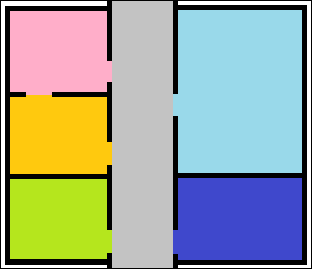
\includegraphics[width=\linewidth]{layout_alg}
	\captionof{figure}{Basisillustratie opstelling}
	\label{fig:ops-basis}
\end{minipage}

\section[RFID]{De RFID opstellingen}
\label{sec:ops-rfid}

\subsection{Statisch}
\subsubsection{1 antenne aan deurlijst}
\begin{minipage}{0.65\textwidth}
Deze opstelling is de eenvoudigste en is 1 van de opstellingen die momenteel wordt gebruikt door Aucxis, ze is voornamelijk opgenomen in dit onderzoek ter referentie. Het concept bij deze opstelling is dat aan elke deurlijst 1 RFID antenne hangt. Als er een tag voorbij de antenne komt registreert deze dit is er een beweging gedetecteerd. Of deze in of uit de locatie is kan niet uit deze data alleen afgeleid worden, dit kan enkel in combinatie met de informatie wat zijn locatie was voor de verplaatsing. Deze opstelling staat geïllustreerd op figuur~\ref{fig:ops-rfid-static-1}.
\end{minipage}
\hfill
\begin{minipage}{0.30\textwidth}
	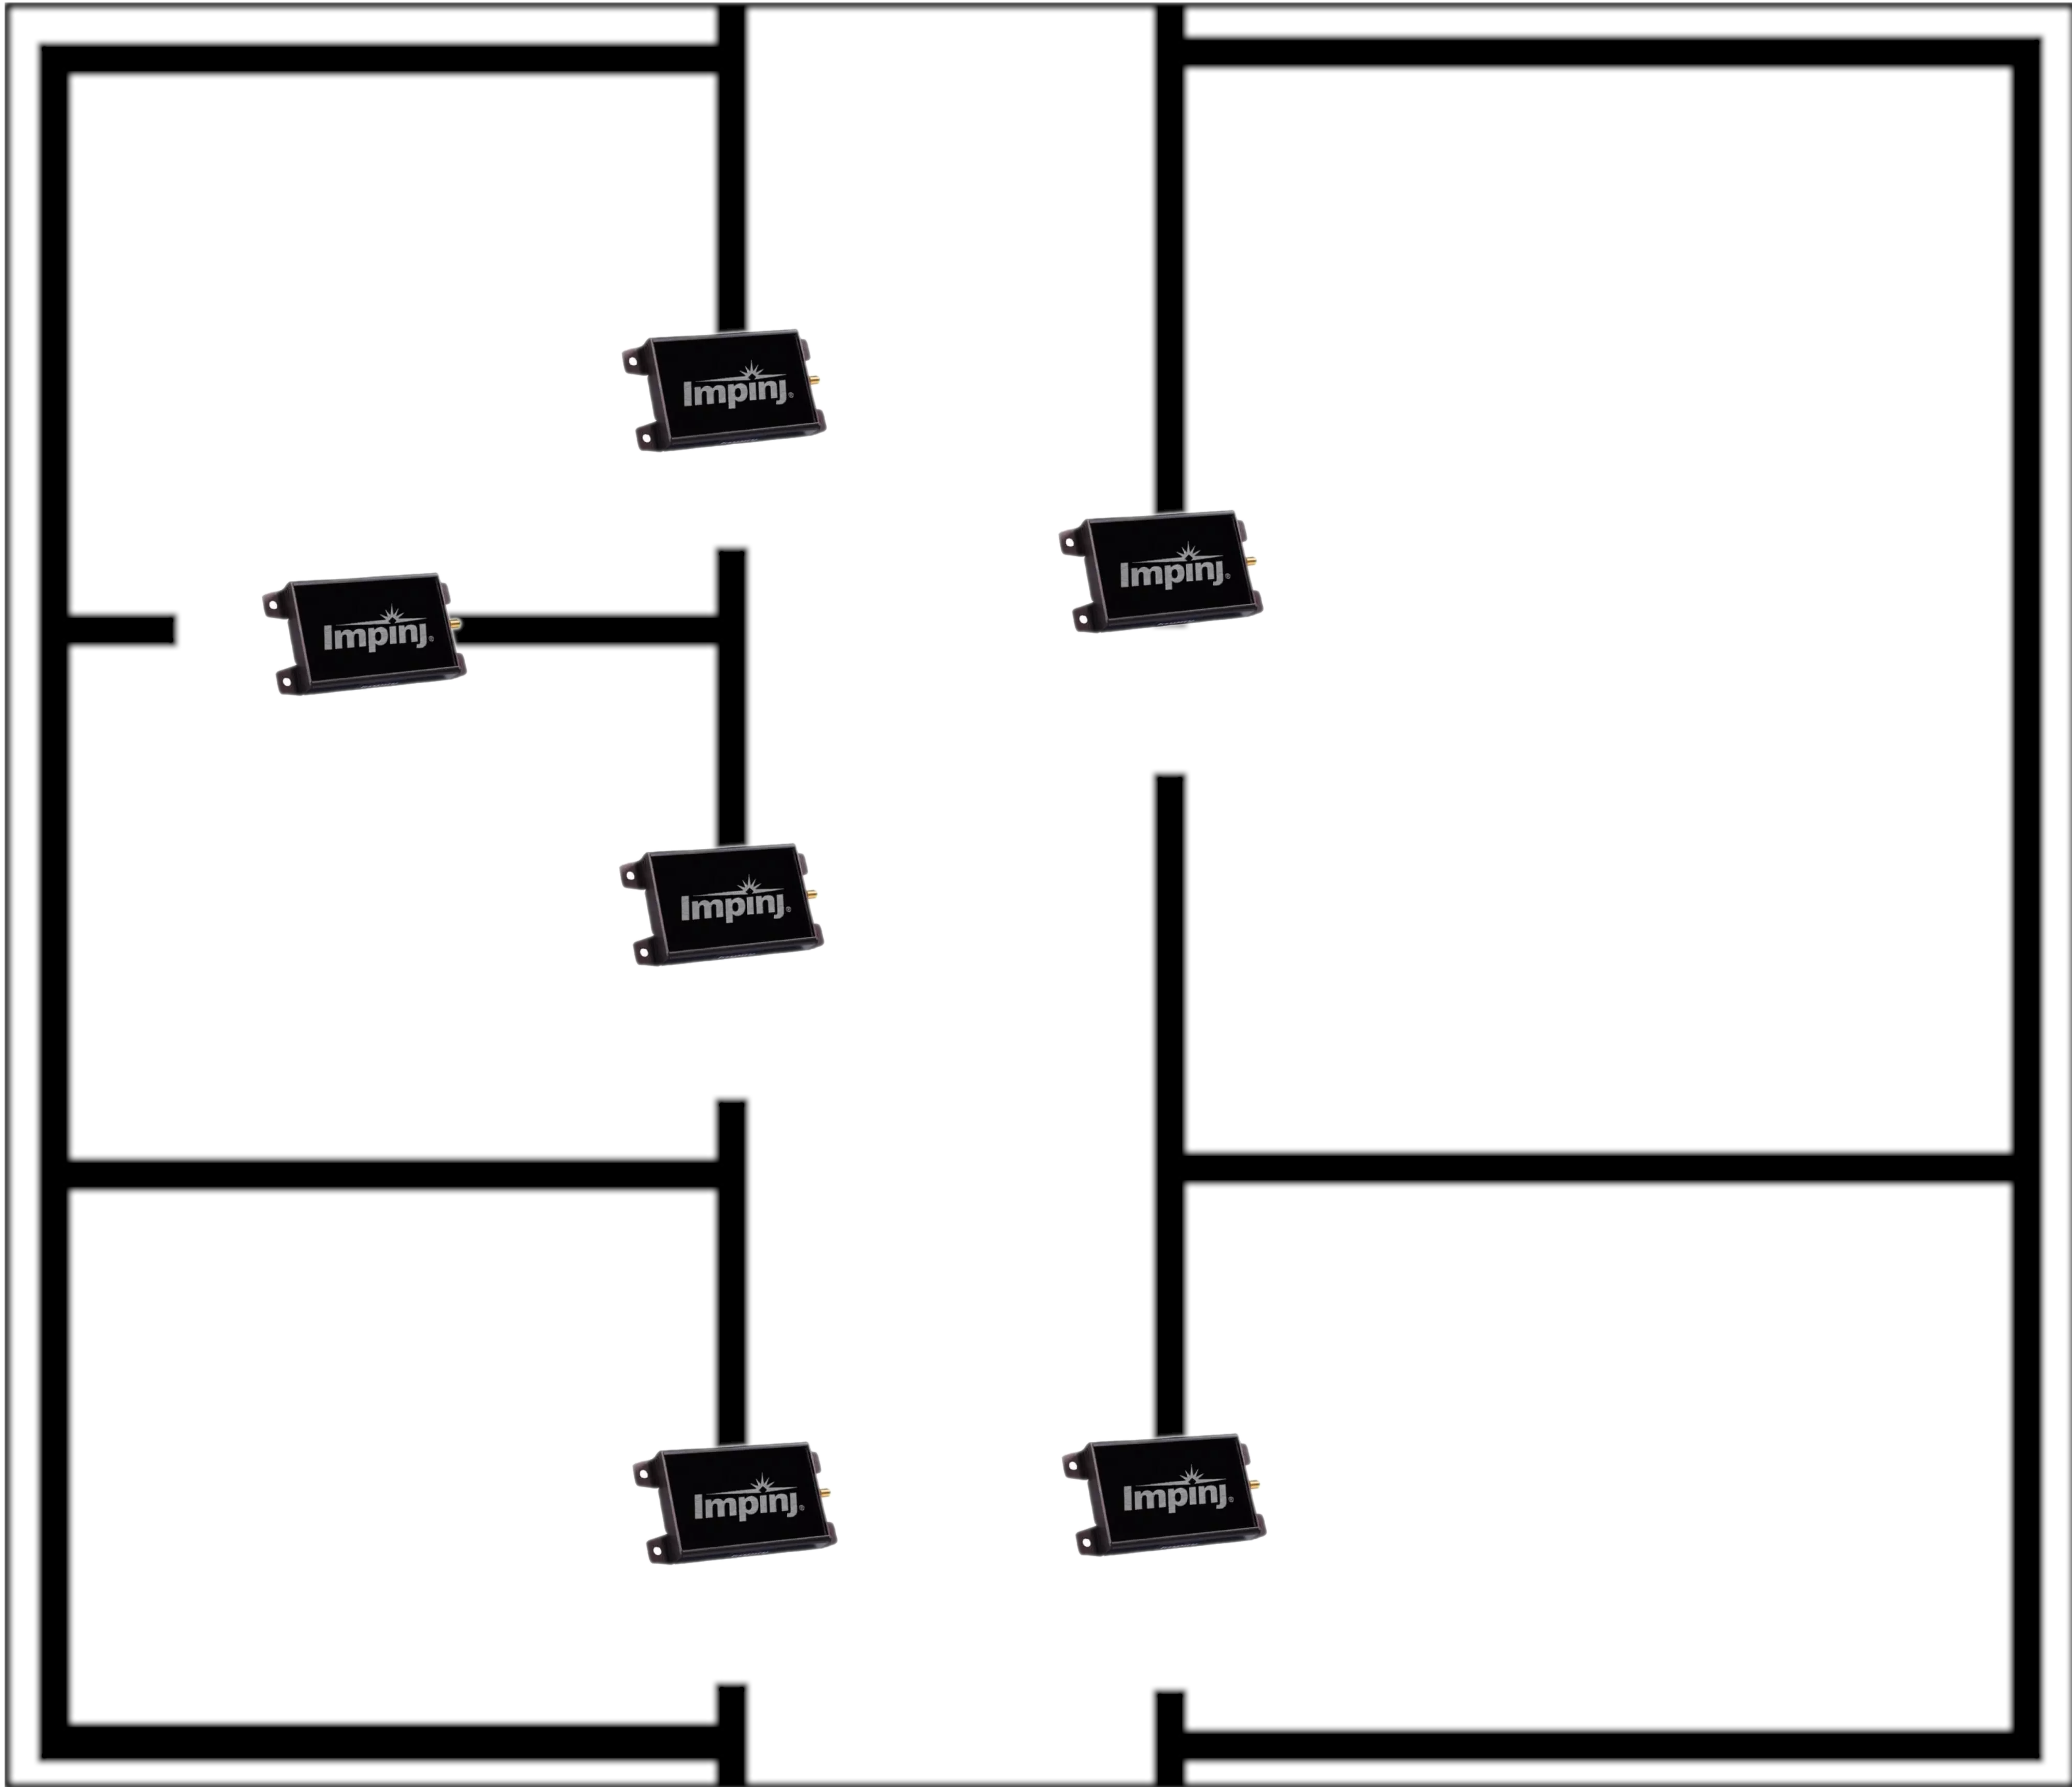
\includegraphics[width=\linewidth]{rfid_static_1}
	\captionof{figure}{Illustratie 1 antenne aan deurlijst}
	\label{fig:ops-rfid-static-1}
\end{minipage}

\subsubsection{2 antennes aan deurlijst}
\begin{minipage}{0.65\textwidth}
Ook dit is 1 van de opstellingen die momenteel wordt gebruikt door Aucxis en is ook voornamelijk een referentiepunt. Het principe is hetzelfde als bij de vorige opstelling, echter is het voordeel hier dat de richting van de verplaatsing wel bekend is, dit aan de hand van het tijdsverschil tussen de detecties van de tag. In dit opzicht is het beter dan de vorige opstelling, maar is uiteraard duurder door de hogere aantallen benodigde antennes en de extra benodigde poorten in de transceivers. Deze opstelling staat geïllustreerd op figuur~\ref{fig:ops-rfid-static-2}.
\end{minipage}
\hfill
\begin{minipage}{0.30\textwidth}
	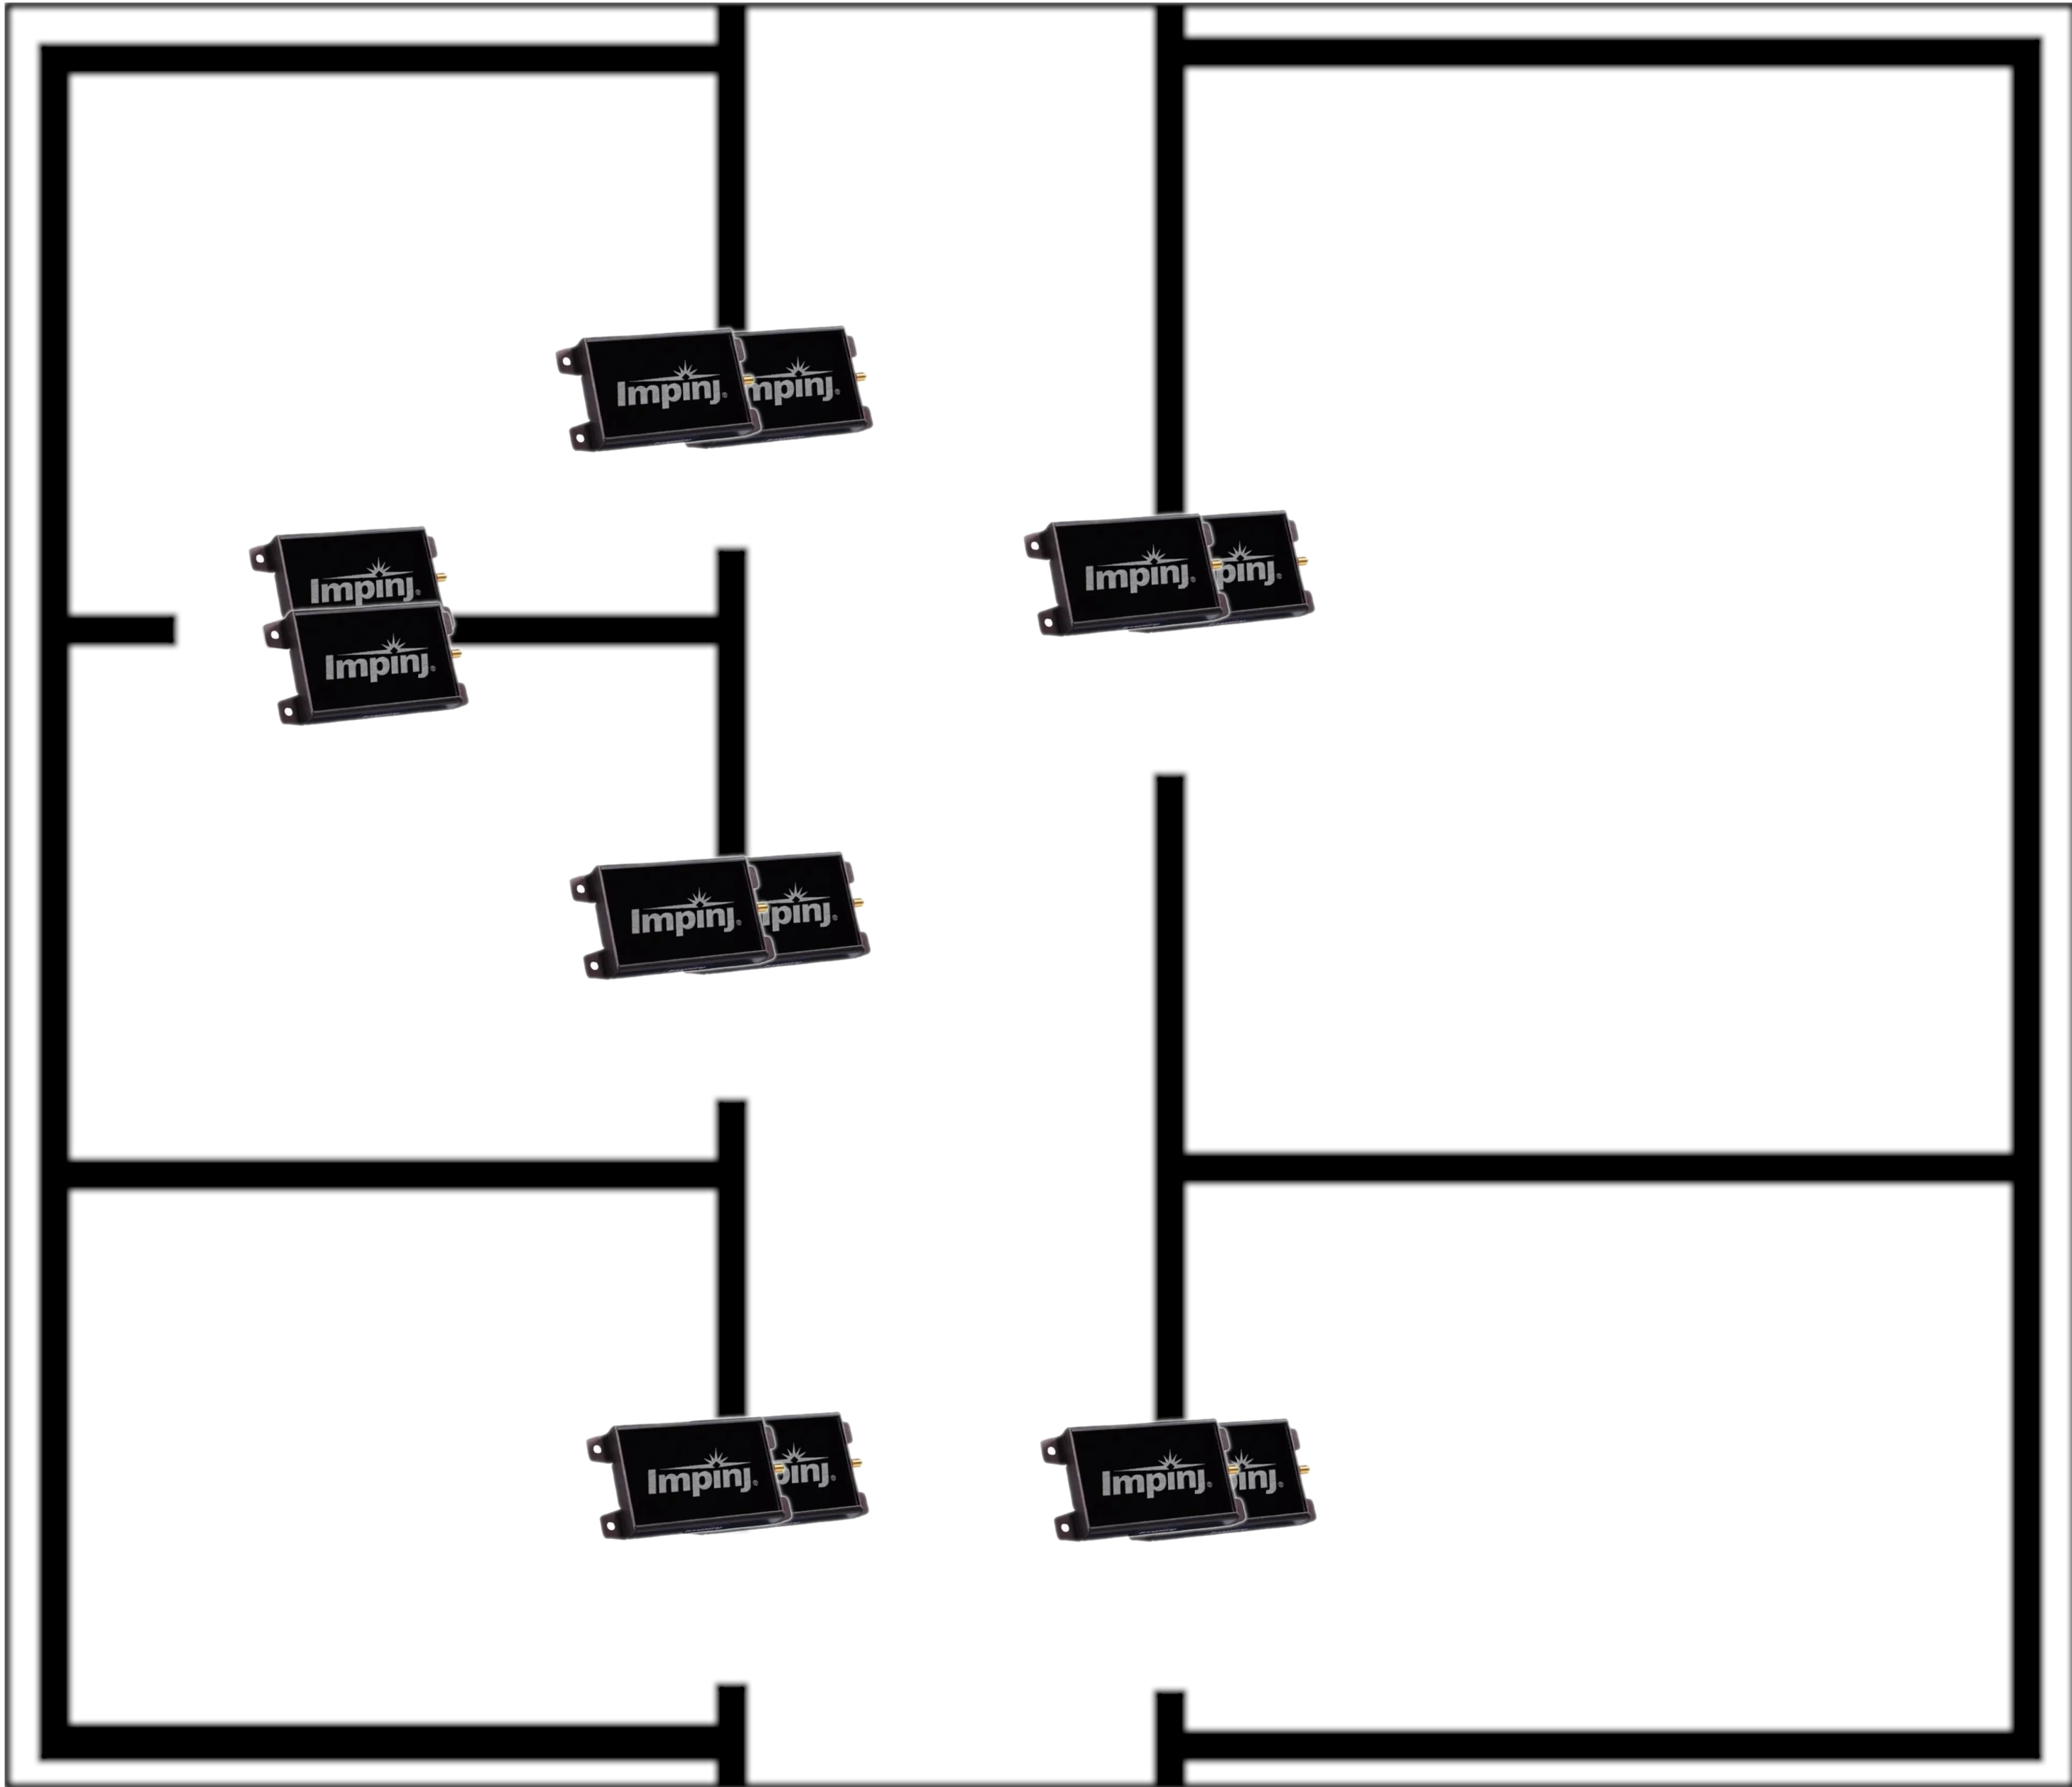
\includegraphics[width=\linewidth]{rfid_static_2}
	\captionof{figure}{Illustratie 2 antennes aan deurlijst}
	\label{fig:ops-rfid-static-2}
\end{minipage}

\subsubsection{1 antenne tegenover deur}
\begin{minipage}{0.65\textwidth}
Bij deze opstelling wordt een RFID antenne tegenover de deur geplaatst. Het idee hierachter is het feit dat, aangezien de RSSI afhankelijk is van de afstand tussen de antenne en de tag, het in theorie zichtbaar is aan de verandering in RSSI in welke richting de tag gaat. Ook geeft de antenne een doppler waarde mee, welke in theorie ook veranderd naargelang de richting. Als dit in praktijk blijkt te werken wilt dit zeggen dat er richtingsdetectie mogelijk is met 1 antenne, waardoor het sowieso al beter is dan de vorige 2 opstellingen. De verwachting is wel dat de kamer niet te breed mag zijn, zodat de antenne van de gemonteerde antenne tot de deur niet te groot is. Deze opstelling staat geïllustreerd op figuur~\ref{fig:ops-rfid-static-3}.
\end{minipage}
\hfill
\begin{minipage}{0.30\textwidth}
	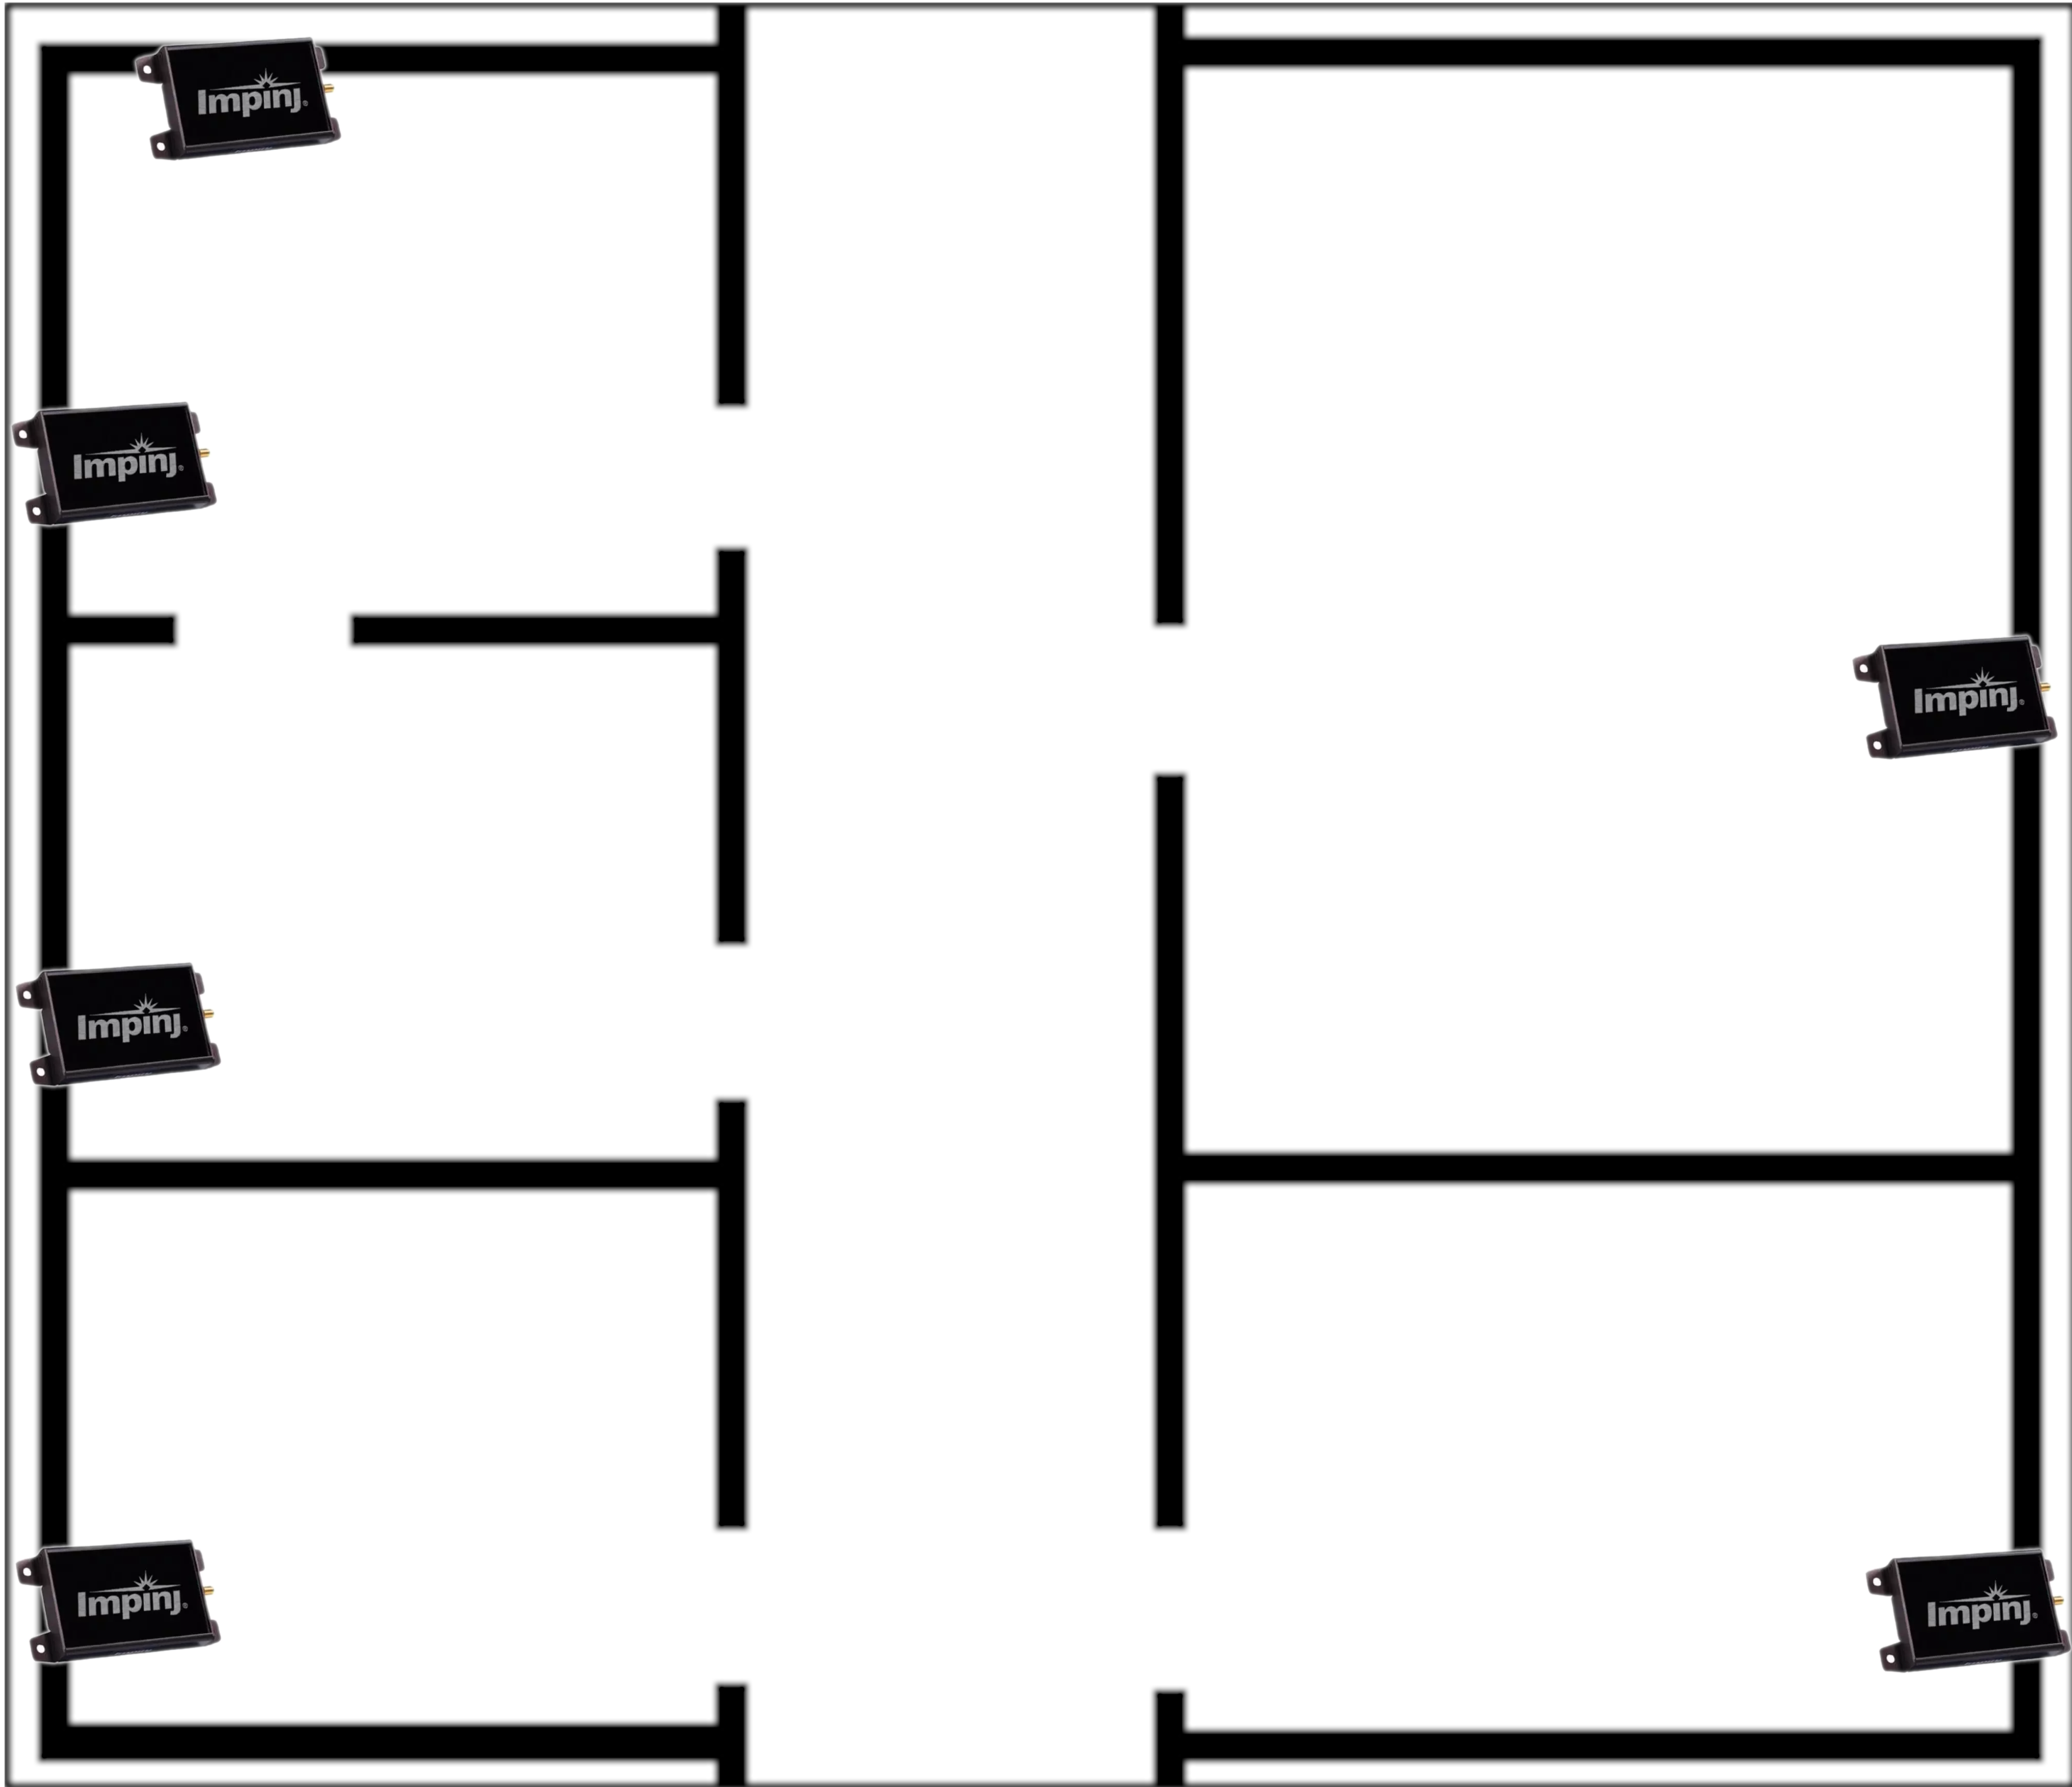
\includegraphics[width=\linewidth]{rfid_static_3}
	\captionof{figure}{Illustratie 1 antenne tegenover deur}
	\label{fig:ops-rfid-static-3}
\end{minipage}
\subsection{Dynamisch}

\subsubsection{1 tag aan deurlijst}
\begin{minipage}{0.65\textwidth}
Hier hangt er een RFID-tag aan de deurlijst (analoog aan de antenne bij de eerste statische opstelling). Als de antenne passeert aan de deur weet het aggregatieprogramma in theorie dat alle tags tussen nu en het voorbijkomen van deze of een andere locatie tag tot deze locatie behoren. Om dit te kunnen weten is ook een opsplitsing in de RFID-tags nodig, nl. of het een locatie of een asset tag is. Deze opstelling staat geïllustreerd op figuur~\ref{fig:ops-rfid-dynamic-1}.
\end{minipage}
\hfill
\begin{minipage}{0.30\textwidth}
	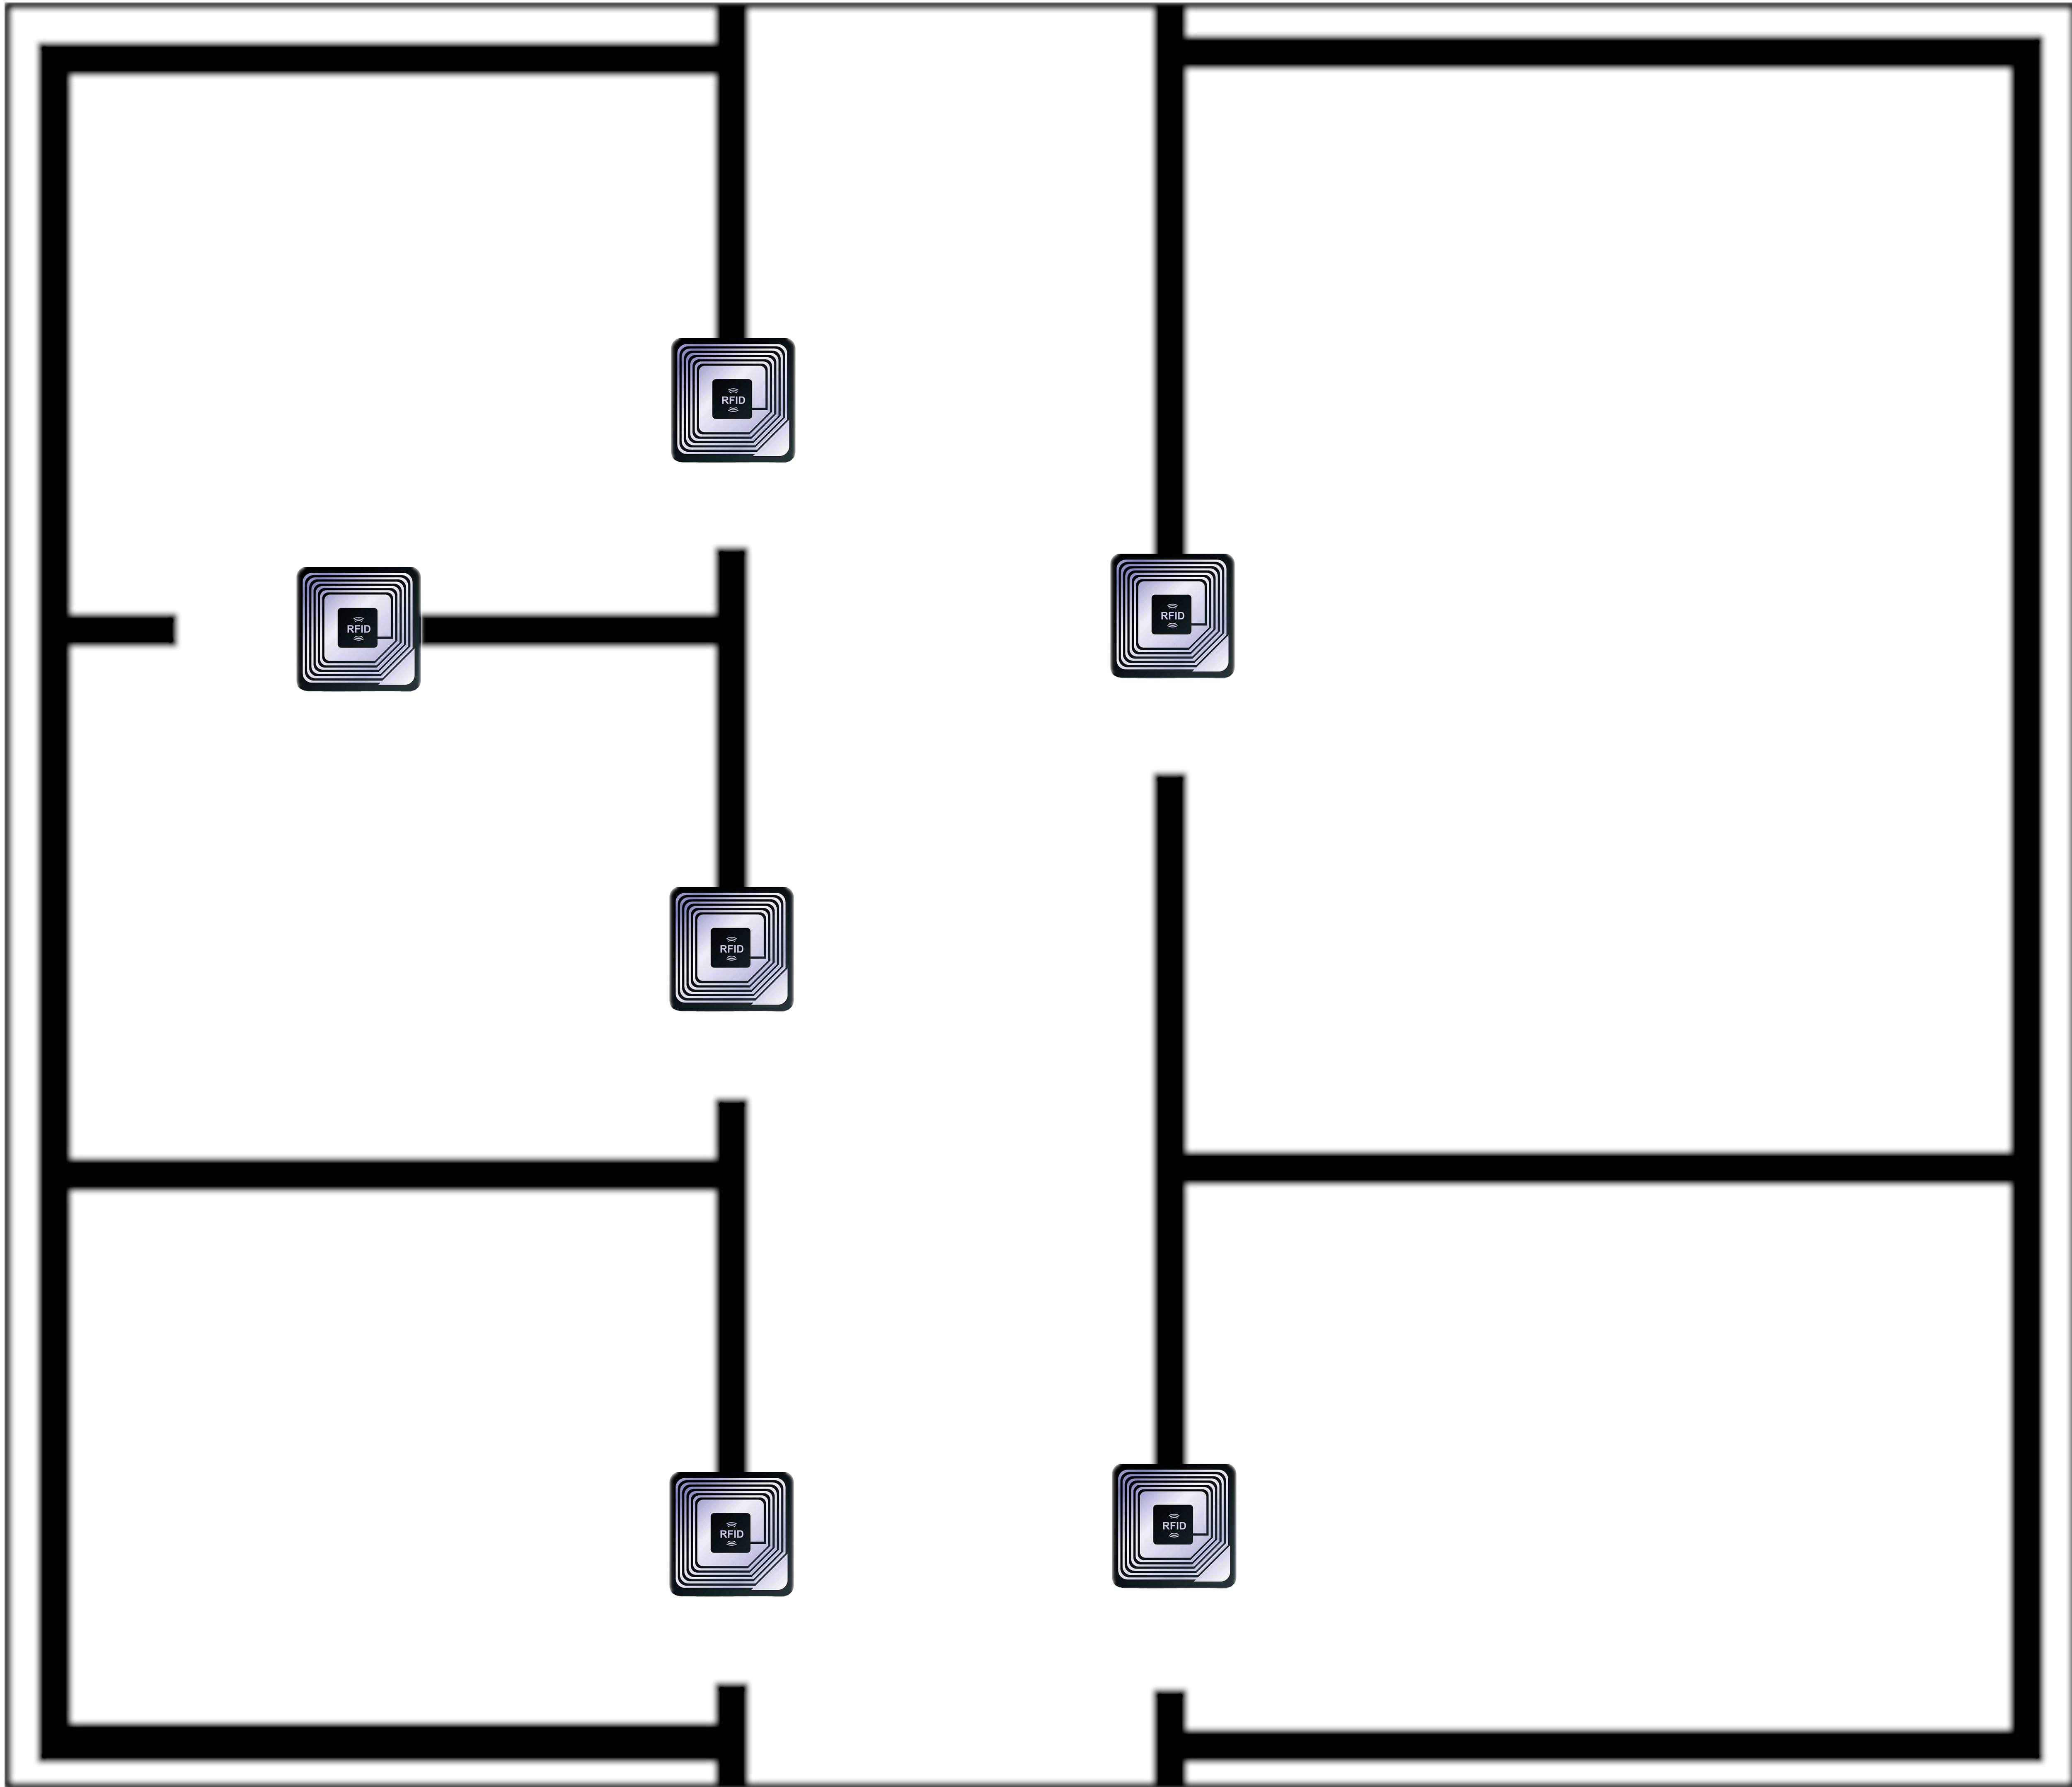
\includegraphics[width=\linewidth]{rfid_dynamic_1}
	\captionof{figure}{Illustratie 1 tag aan deurlijst}
	\label{fig:ops-rfid-dynamic-1}
\end{minipage}

In theorie is het ook mogelijk de 2 andere statische scenario's een dynamische variant te geven, echter valt hun voordeel van richtingbepalend zijn weg hierbij doordat de detectie richting niet meer zo nuttig is bij een dynamische opstelling, aangezien door de aard van dit type opstelling de tijd belangrijker wordt en de real-time grotendeels wegvalt, waardoor er informatie van meer meetpunten, en bijgevolg volgordes in de tijd beschikbaar is.

\section[BLE]{De BLE opstellingen}
\label{sec:ops-ble}

\subsection{Statisch}

\subsubsection{1 gateway per locatie}
\begin{minipage}{0.65\textwidth}
Deze opstelling is de eenvoudigste en meest intuïtieve van de BLE opstellingen. Elke locatie komt overeen met 1 IoT Gateway, die gepositioneerd wordt in het middelpunt van de locatie. Het idee hierachter is dat de Gateway waar de beacon zich het dichtste bij bevind, en de hoogste RSSI waarde heeft, de locatie is waar het voorwerp zich bevind. Echter is de verwachting dat dit niet volledig zal kloppen, en dat er hier zeker onnauwkeurigheden zullen ontstaan, specifiek als de locaties niet evenredig verdeeld zijn over het gebouw. Deze opstelling staat geïllustreerd op figuur~\ref{fig:ops-ble-static-1}.
\end{minipage}
\hfill
\begin{minipage}{0.30\textwidth}
	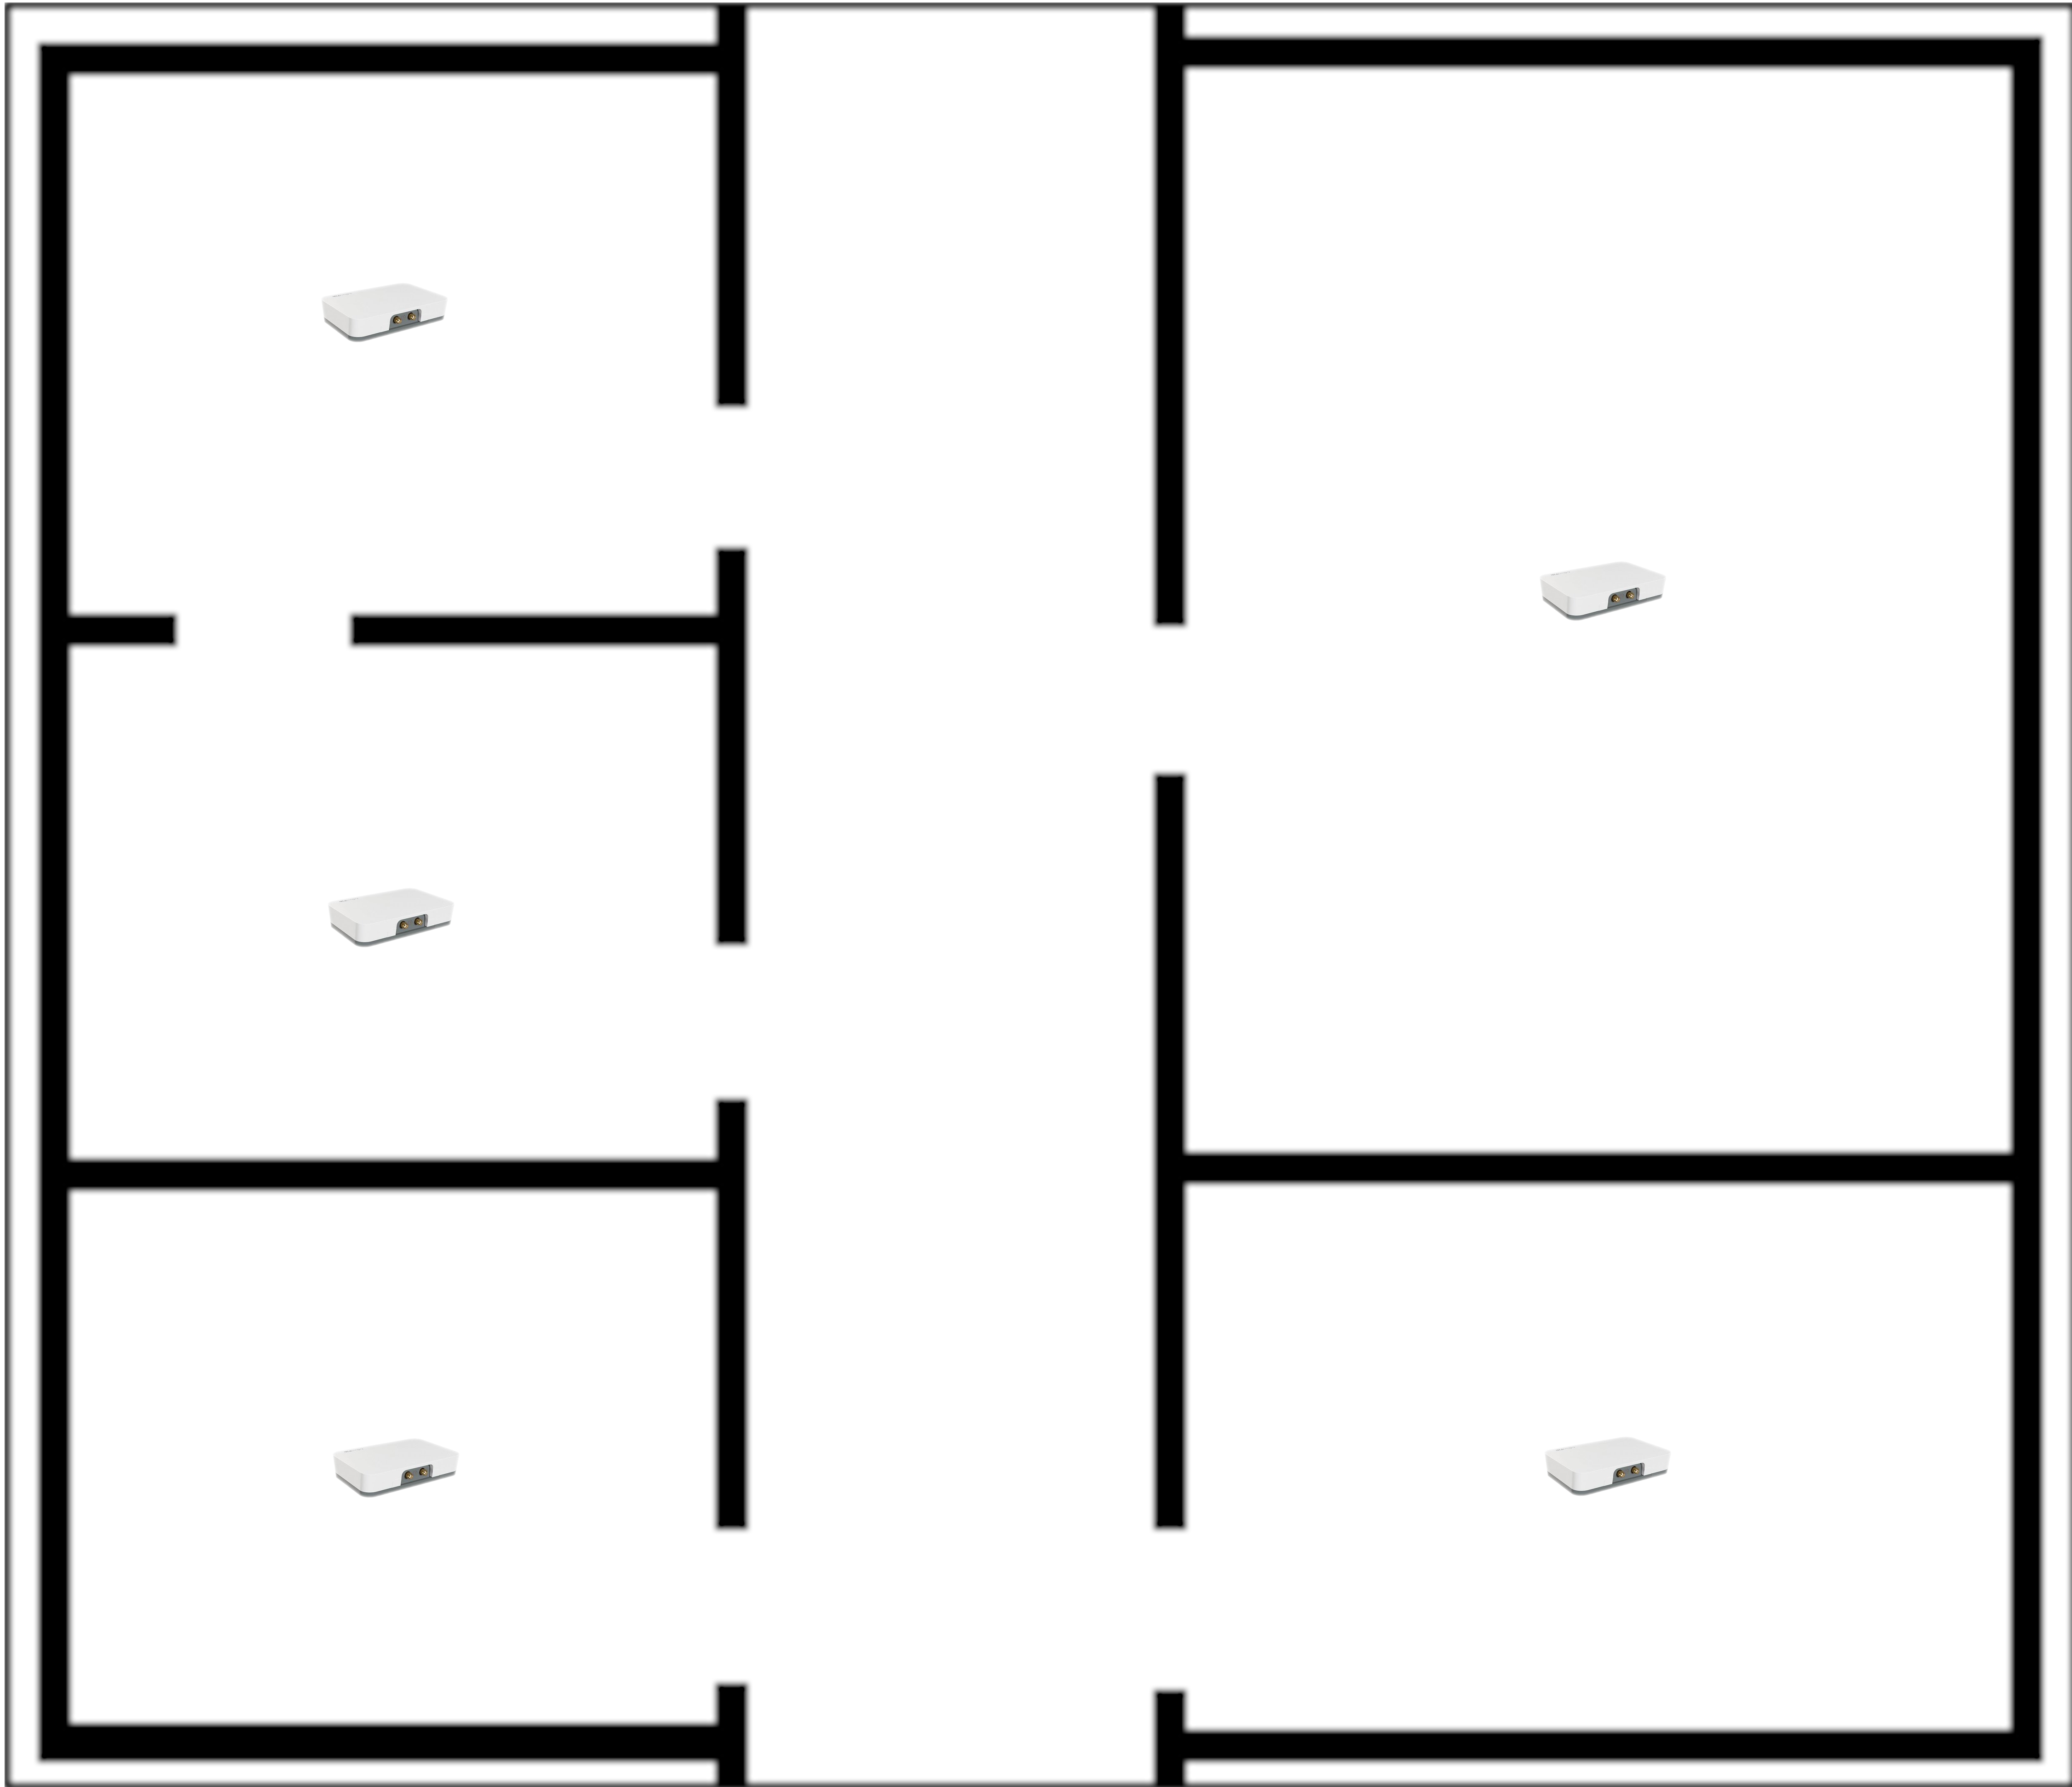
\includegraphics[width=\linewidth]{ble_statisch_1}
	\captionof{figure}{Illustratie 1 gateway per locatie}
	\label{fig:ops-ble-static-1}
\end{minipage}

\subsubsection{Meerdere gateways per locatie}
\begin{minipage}{0.65\textwidth}
In deze opstelling wordt een locatie gedefinieerd door meer dan 1 gateway, nl. een gateway per hoek van de locatie, zodat de locatie wordt omringd door een kader van gateways. Het idee hierbij is dat er aan de data kan afgeleid worden of de beacon zich al dan niet in het vak tussen de gateways bevind, dit door een principe van hoogste som van RSSI-waardes. Echter zal de kost voor de opstelling vrij snel de hoogte in vliegen als er veel locaties zijn. Wel kunnen gedeelde hoeken van locaties door een gedeelde beacon worden bezet, wat ook zo zal zijn in de testopstellingen. Deze opstelling staat geïllustreerd op figuur~\ref{fig:ops-ble-static-2}.
\end{minipage}
\hfill
\begin{minipage}{0.30\textwidth}
	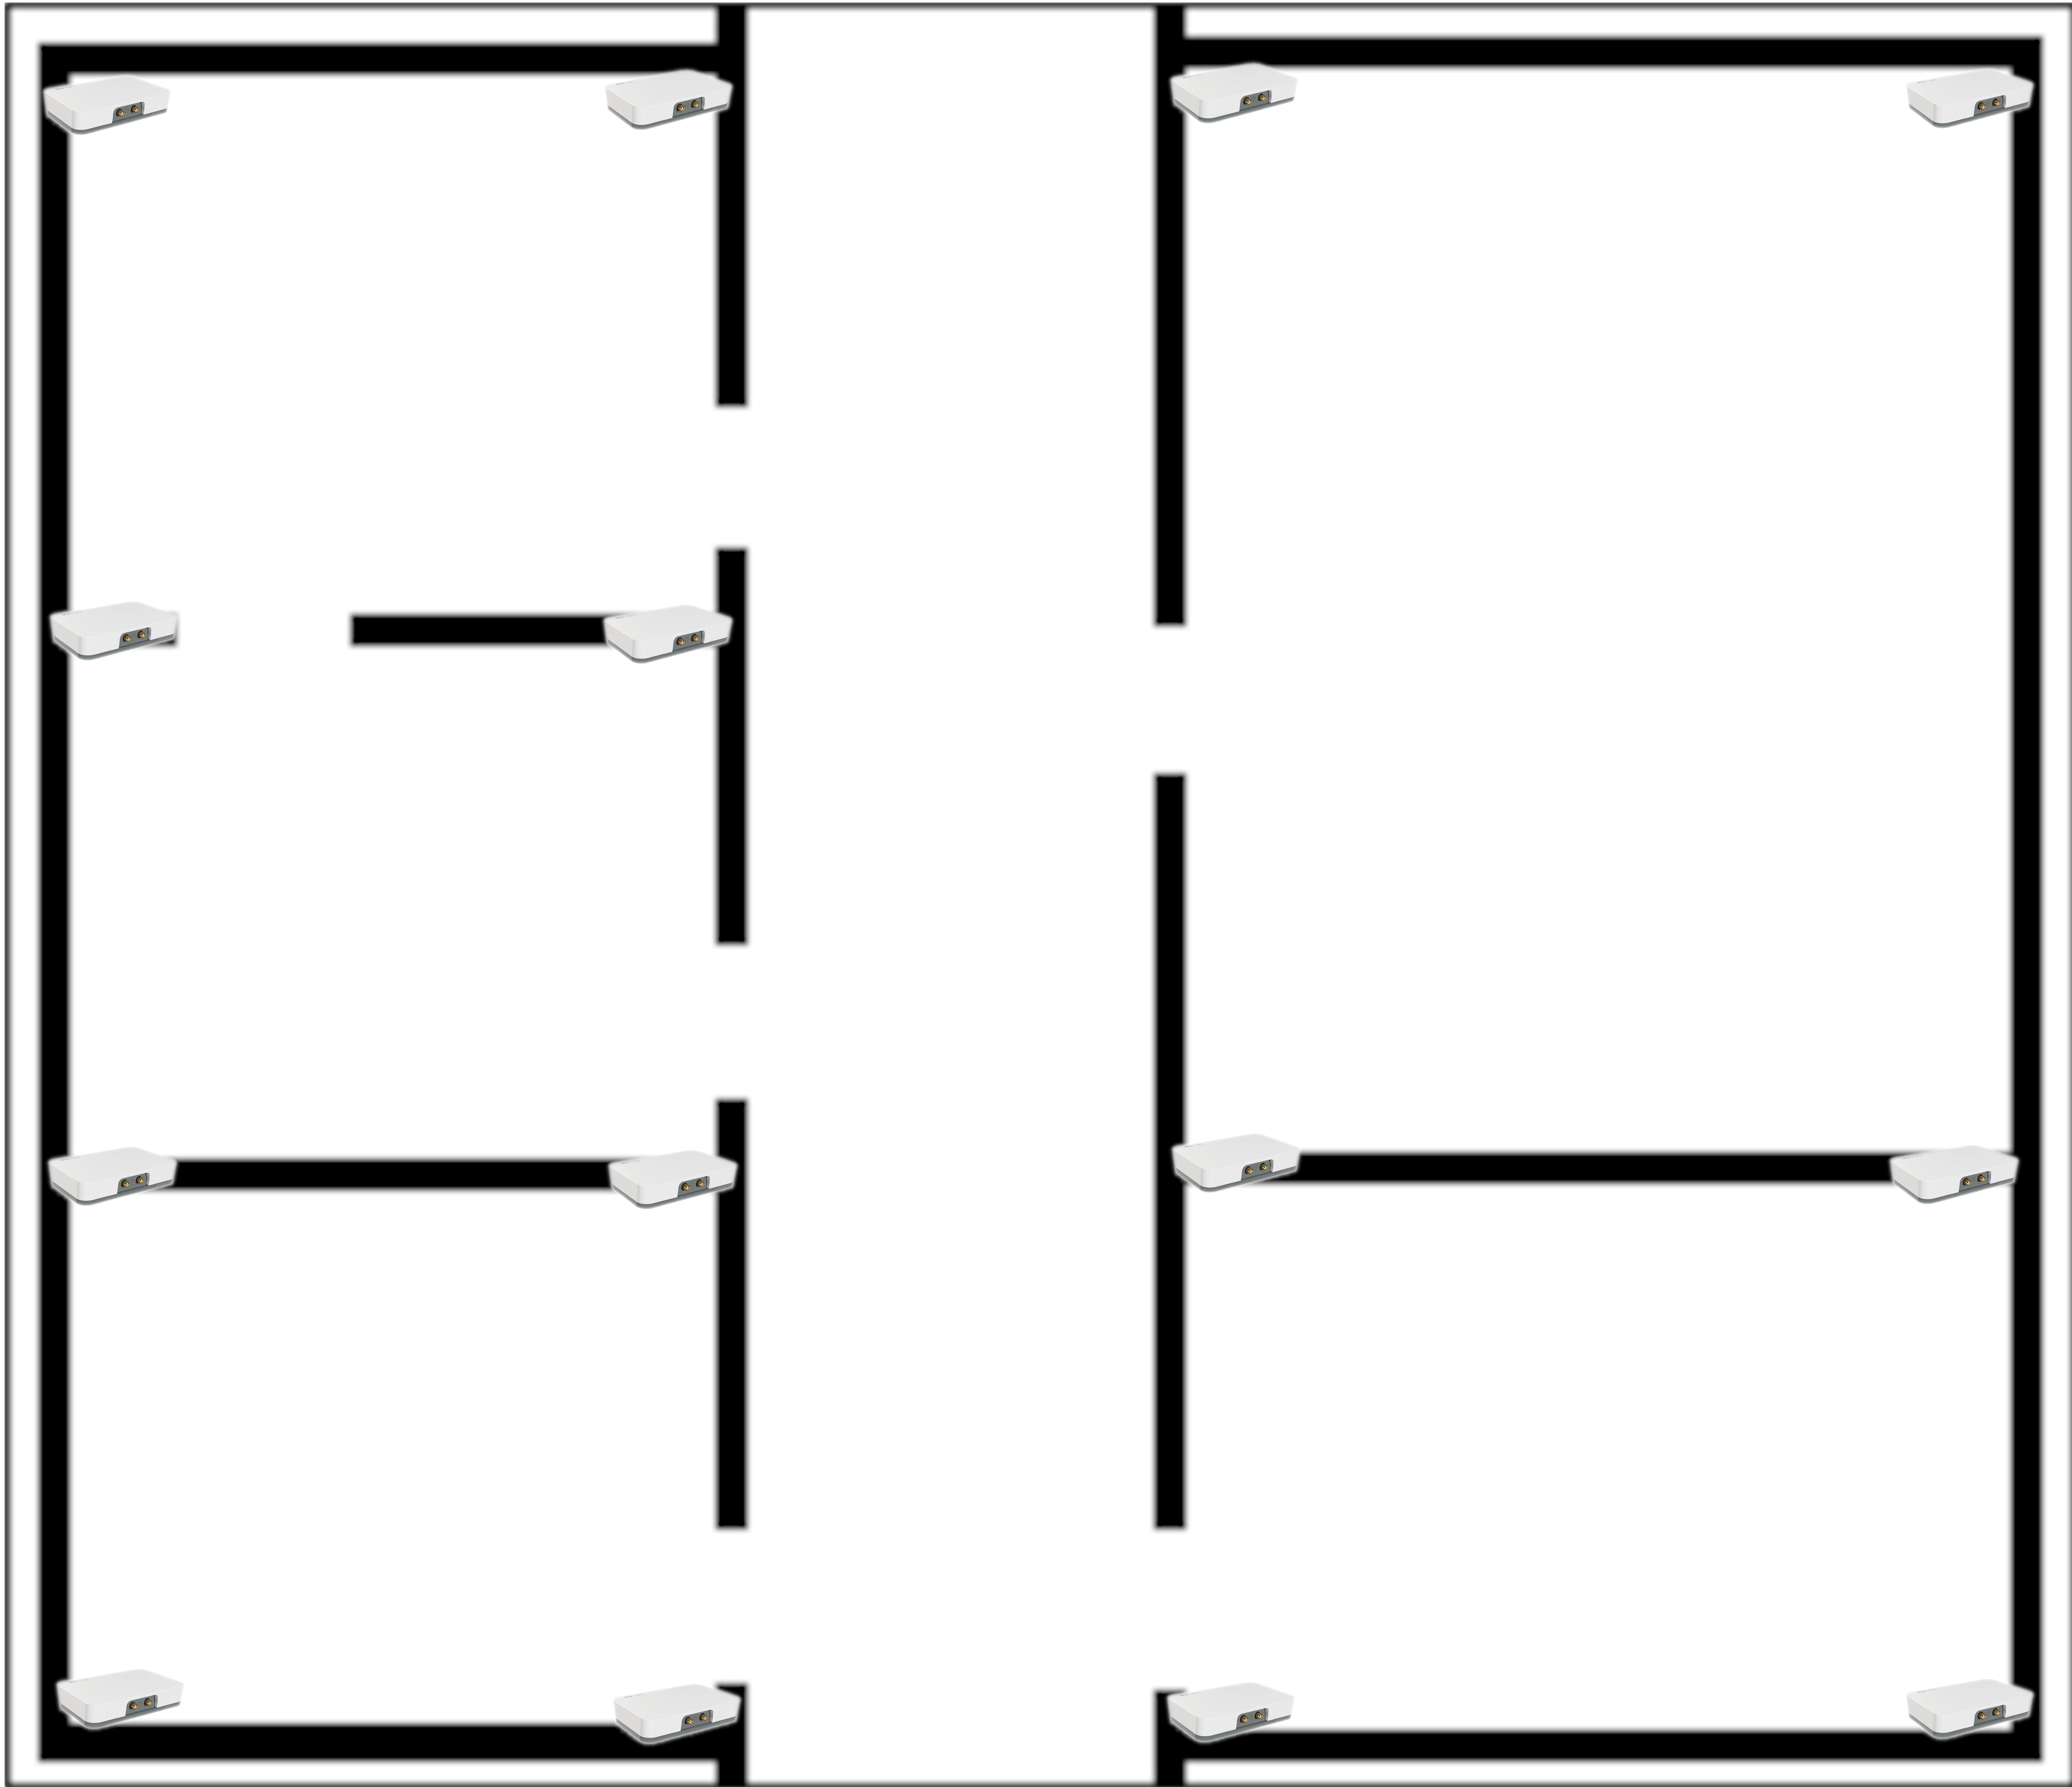
\includegraphics[width=\linewidth]{ble_statisch_2}
	\captionof{figure}{Illustratie meerdere gateways per locatie}
	\label{fig:ops-ble-static-2}
\end{minipage}

\subsubsection{Gateways in rasteropstelling}
\begin{minipage}{0.65\textwidth}
Deze opstelling bestaat uit een raster welke volledig het gebouw omvat. Als de locaties van deze gateways bekend zijn kan via trilateratie\footnotemark met de gemeten RSSI waardes berekend worden waar de voorwerpen zich bevinden, wat dan gelinkt kan worden aan een locatie. De verwachting is dat hiermee de locatie vrij specifiek kan worden bepaald, maar nadelig is wel er meer data zal moeten bijgehouden worden, zoals definities van de locaties in het raster etc. Daardoor kan er niet enkel op data van de gateways worden afgegaan om de locatie te bepalen aangezien in de opstelling de gateways en de locaties niks met elkaar te maken hebben. Deze opstelling lijkt wel meer en eenvoudiger opschaalbaar naar grotere gebouwen of gebouwen met veel dicht bij elkaar liggende locaties. Deze opstelling staat geïllustreerd op figuur~\ref{fig:ops-ble-static-3}.
\end{minipage}
\footnotetext{Zie sectie~\ref{sec:lit-definities} op pagina~\pageref{sec:lit-definities}}
\hfill
\begin{minipage}{0.30\textwidth}
	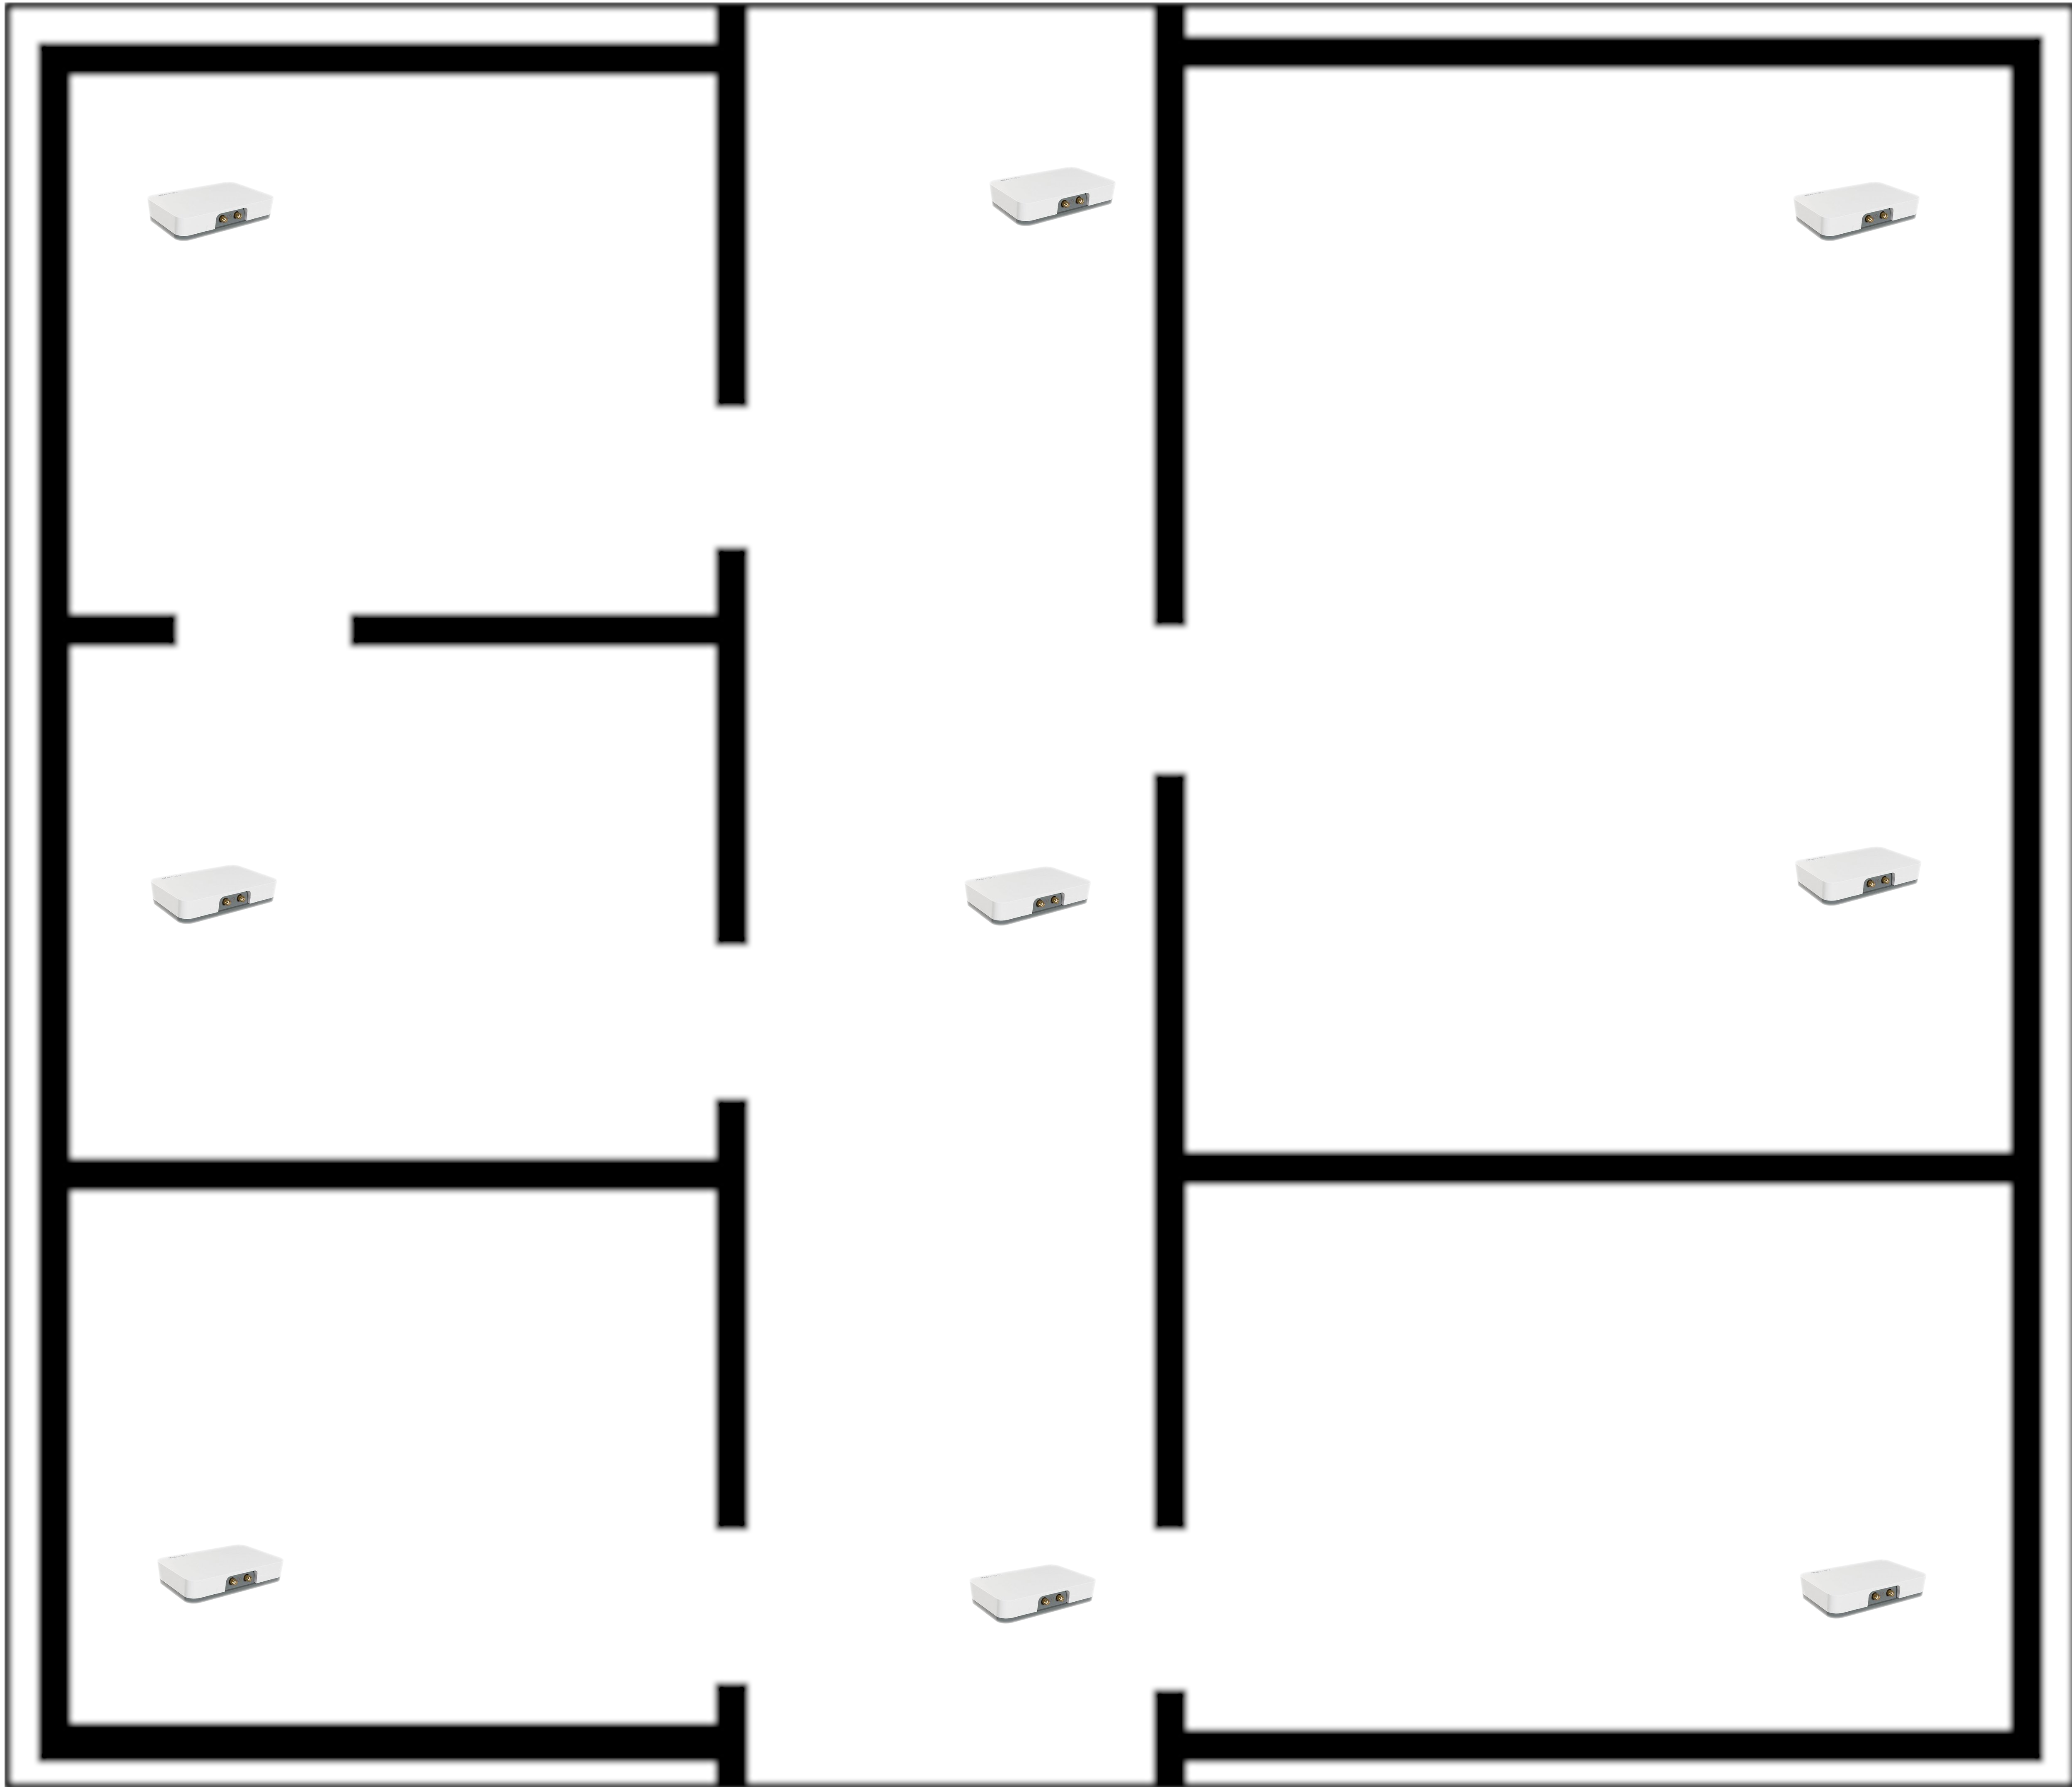
\includegraphics[width=\linewidth]{ble_statisch_3}
	\captionof{figure}{Illustratie gateways in rasteropstelling}
	\label{fig:ops-ble-static-3}
\end{minipage}


\subsection{Dynamisch}

Bij elk van volgende opstellingen zal een onderscheid gemaakt worden in de BLE beacons, nl. de locatie- en de asset-beacons.

\subsubsection{1 beacon per locatie, midden van locatie}
\begin{minipage}{0.65\textwidth}
In deze opstelling bevinden de locatiebeacons zich in het midden van de locatie die ze vertegenwoordigen, voor de categorisatie zal uitgegaan worden van hoogte RSSI. Aangezien de gateway zich enkel in de tussenliggende gang verplaatst, zal het tijdstip waarop de gateway de hoogste RSSI waarde meet het tijdstip zijn waarop deze het dichtste bij de beacon in de buurt is. Hierna kunnen op basis van dicht bij elkaar liggende tijdstippen de assetbeacons toegewezen worden aan een locatie. Deze opstelling staat geïllustreerd op figuur~\ref{fig:ops-ble-dynamic-1}.
\end{minipage}
\hfill
\begin{minipage}{0.30\textwidth}
	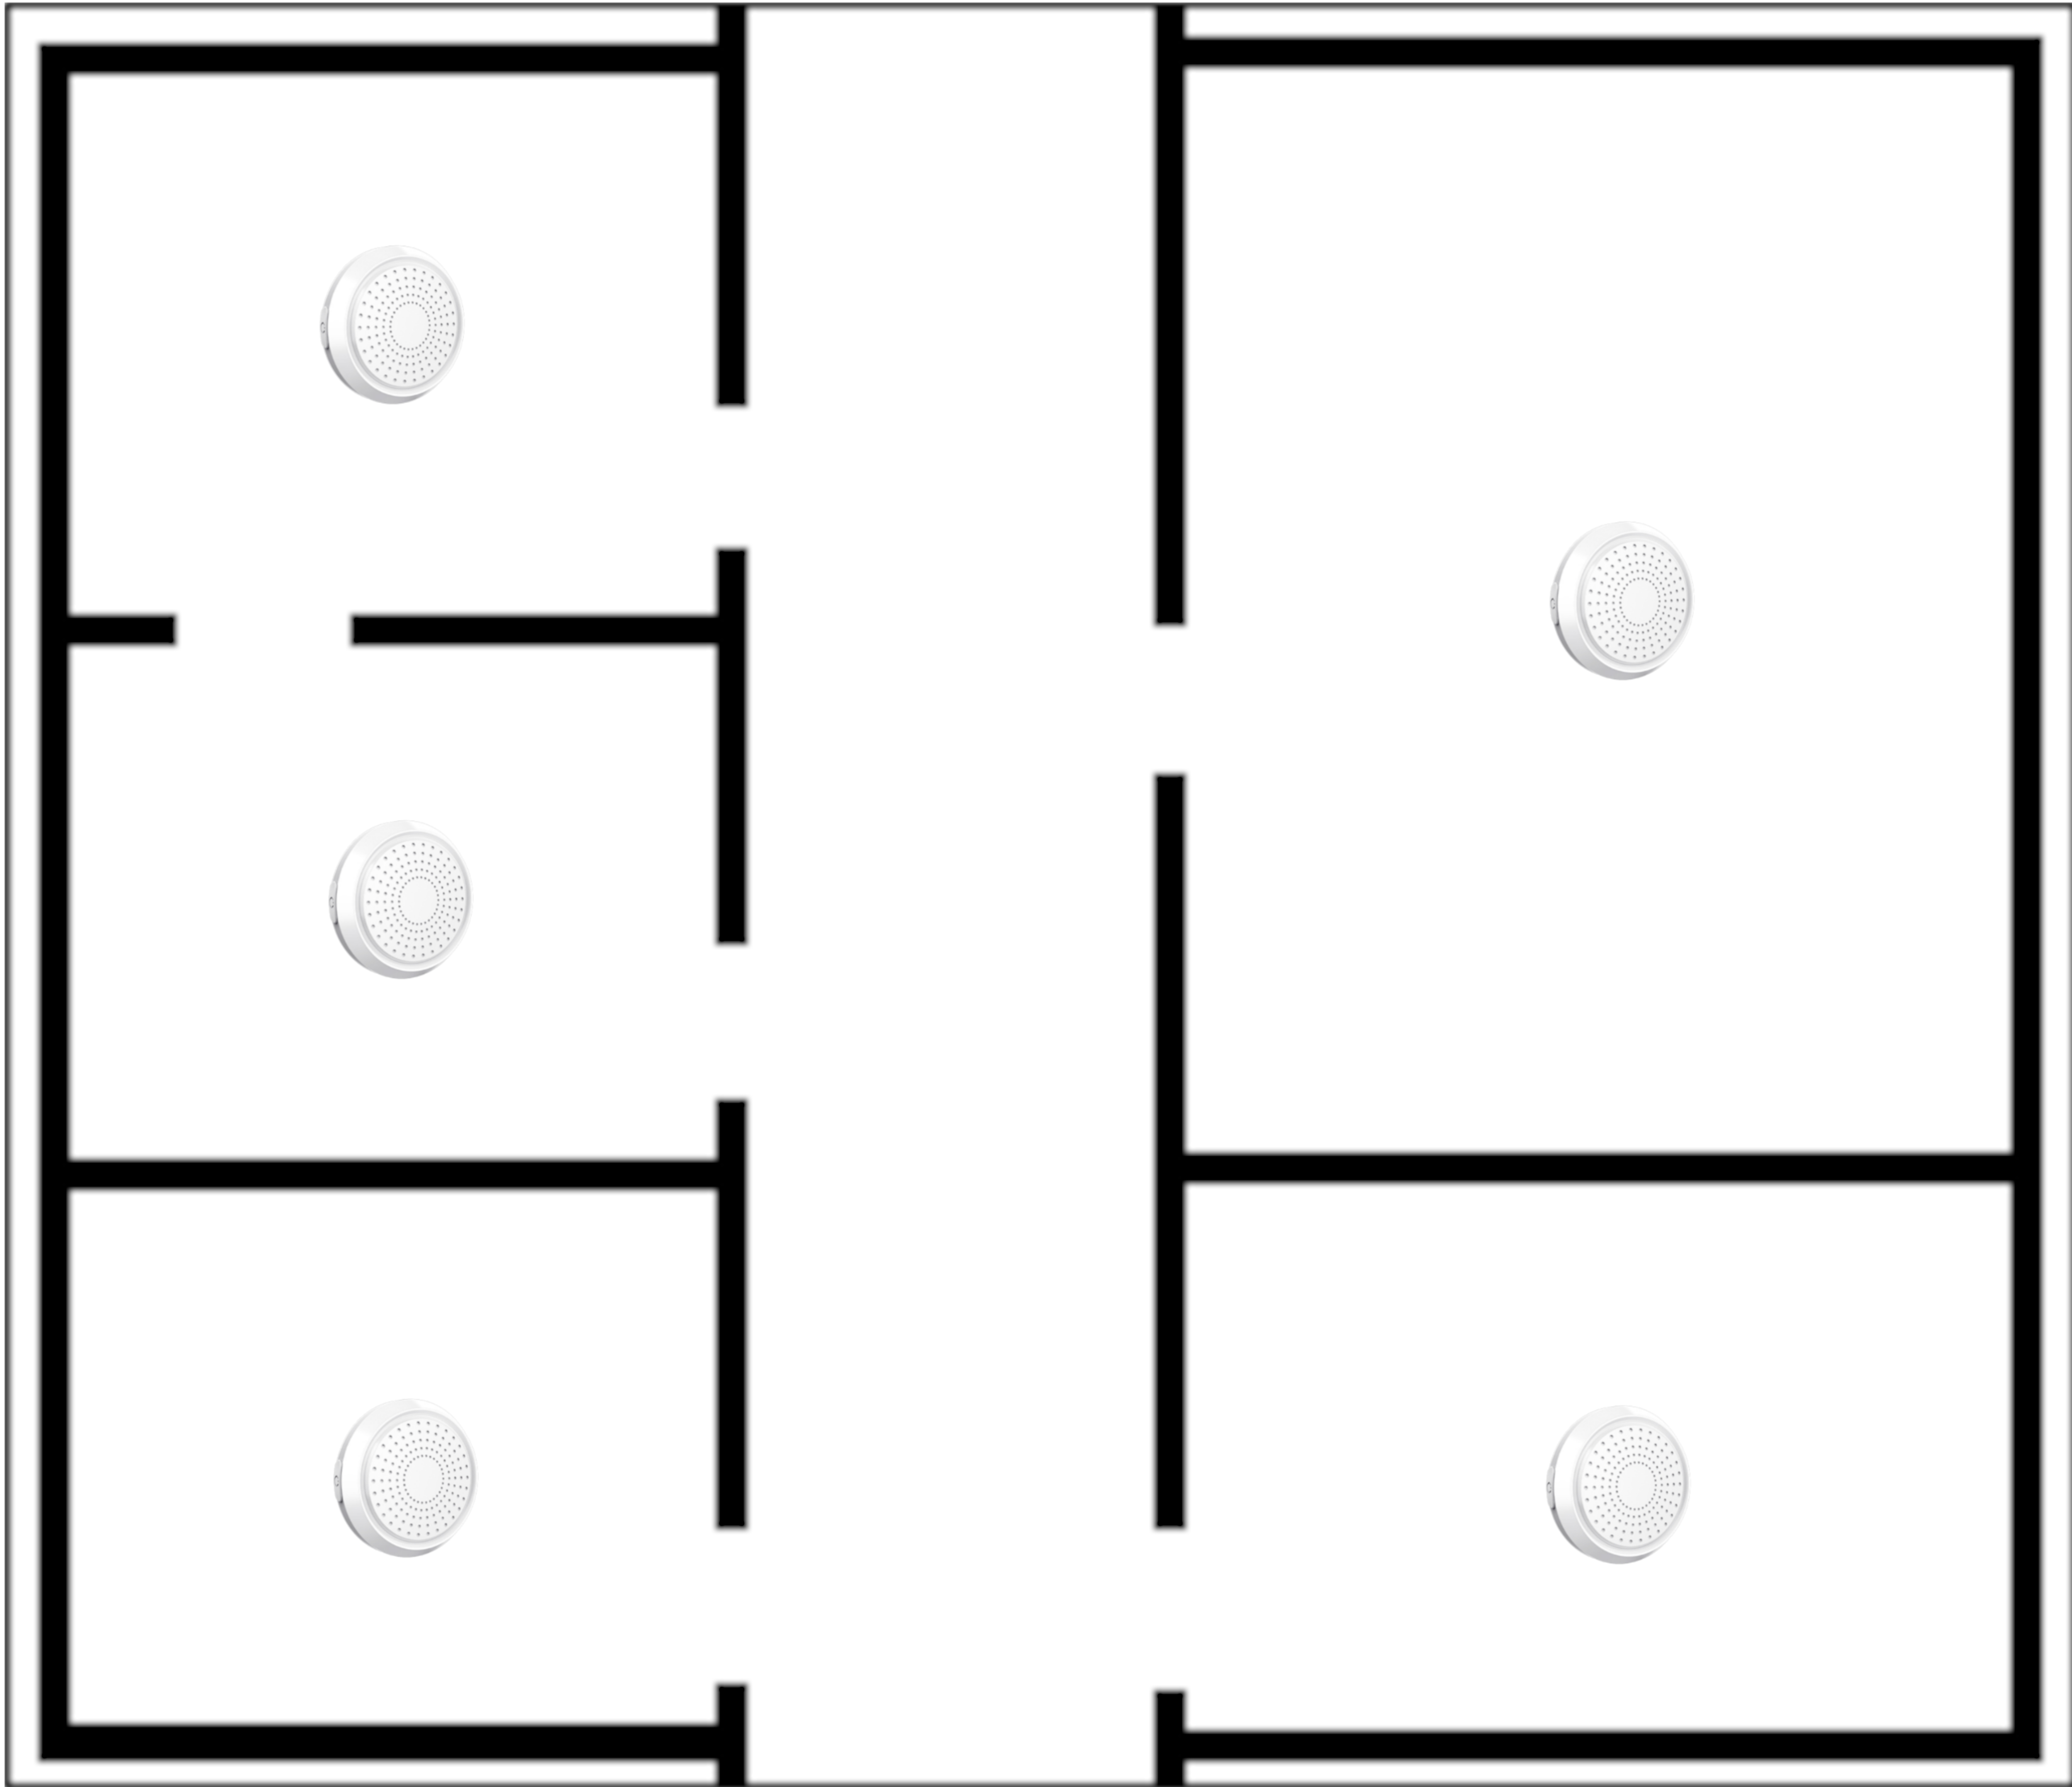
\includegraphics[width=\linewidth]{ble_dynamic_1}
	\captionof{figure}{Illustratie 1 beacon per locatie, midden van locatie}
	\label{fig:ops-ble-dynamic-1}
\end{minipage}

\subsubsection{1 beacon per locatie, aan deur}
\begin{minipage}{0.65\textwidth}
Deze opstelling is qua concept gelijkaardig aan de vorige, het verschil is dat bij deze opstelling de locatiebeacons zich bevinden aan de deur van de locatie/tussen de locatie en de gang. De hypothese is dat hierdoor de mobiele gateway in de gang deze beacon beter kan detecteren, en zijn locatie in de gang beter kan bepalen. Ook is er hier geen beacon aanwezig op de overgang tussen 2 locaties die niet via de gang verloopt, aangezien de mobiele gateway hier niet komt. Deze opstelling staat geïllustreerd op figuur~\ref{fig:ops-ble-dynamic-2}.
\end{minipage}
\hfill
\begin{minipage}{0.30\textwidth}
	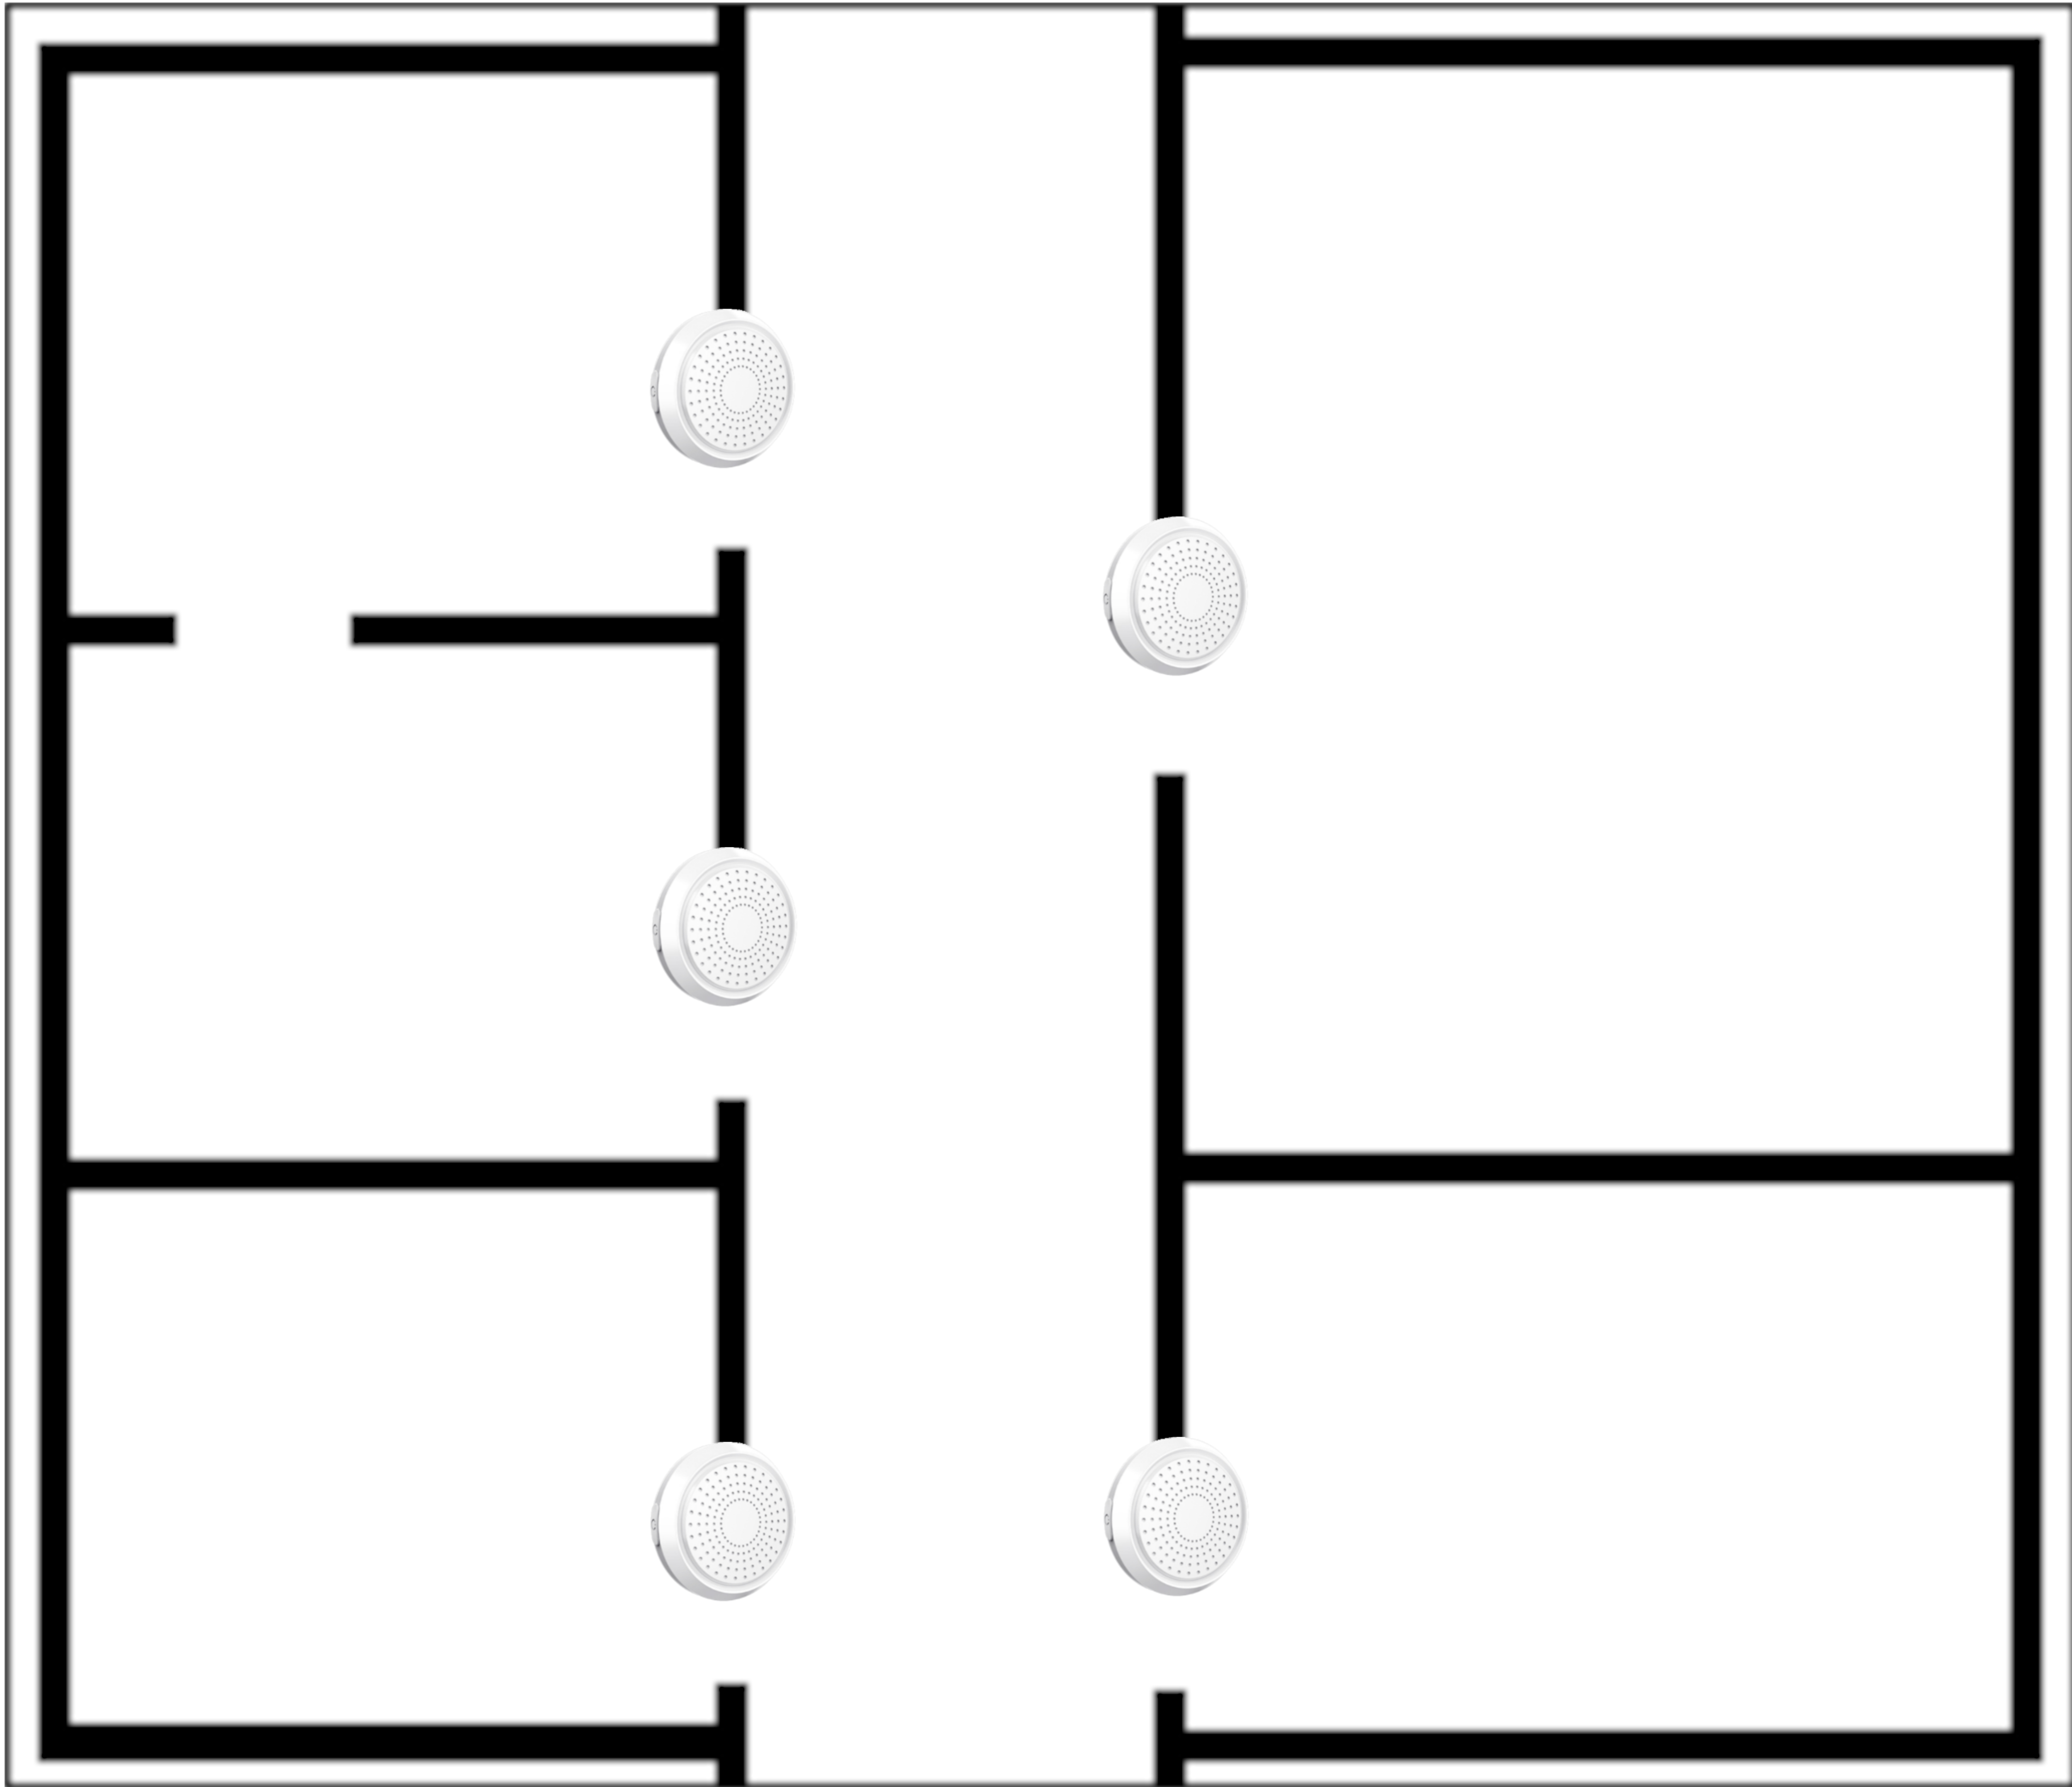
\includegraphics[width=\linewidth]{ble_dynamic_2}
	\captionof{figure}{Illustratie 1 beacon per locatie, aan deur}
	\label{fig:ops-ble-dynamic-2}
\end{minipage}

\subsubsection{Meerdere locatiebeacons per locatie}
\begin{minipage}{0.65\textwidth}
Dit is de dynamische tegenhanger van het 2e statische scenario, echter wordt in dit geval de locatie omringen door locatiebeacons. Hier is het principe dat, als een assetbeacon vanuit verschillende locaties in dezelfde range van RSSI valt als de locatiebeacons van een bepaalde locatie, hij zich waarschijnlijk ook op die locatie zal bevinden. Deze opstelling staat geïllustreerd op figuur~\ref{fig:ops-ble-dynamic-3}.
\end{minipage}
\hfill
\begin{minipage}{0.30\textwidth}
	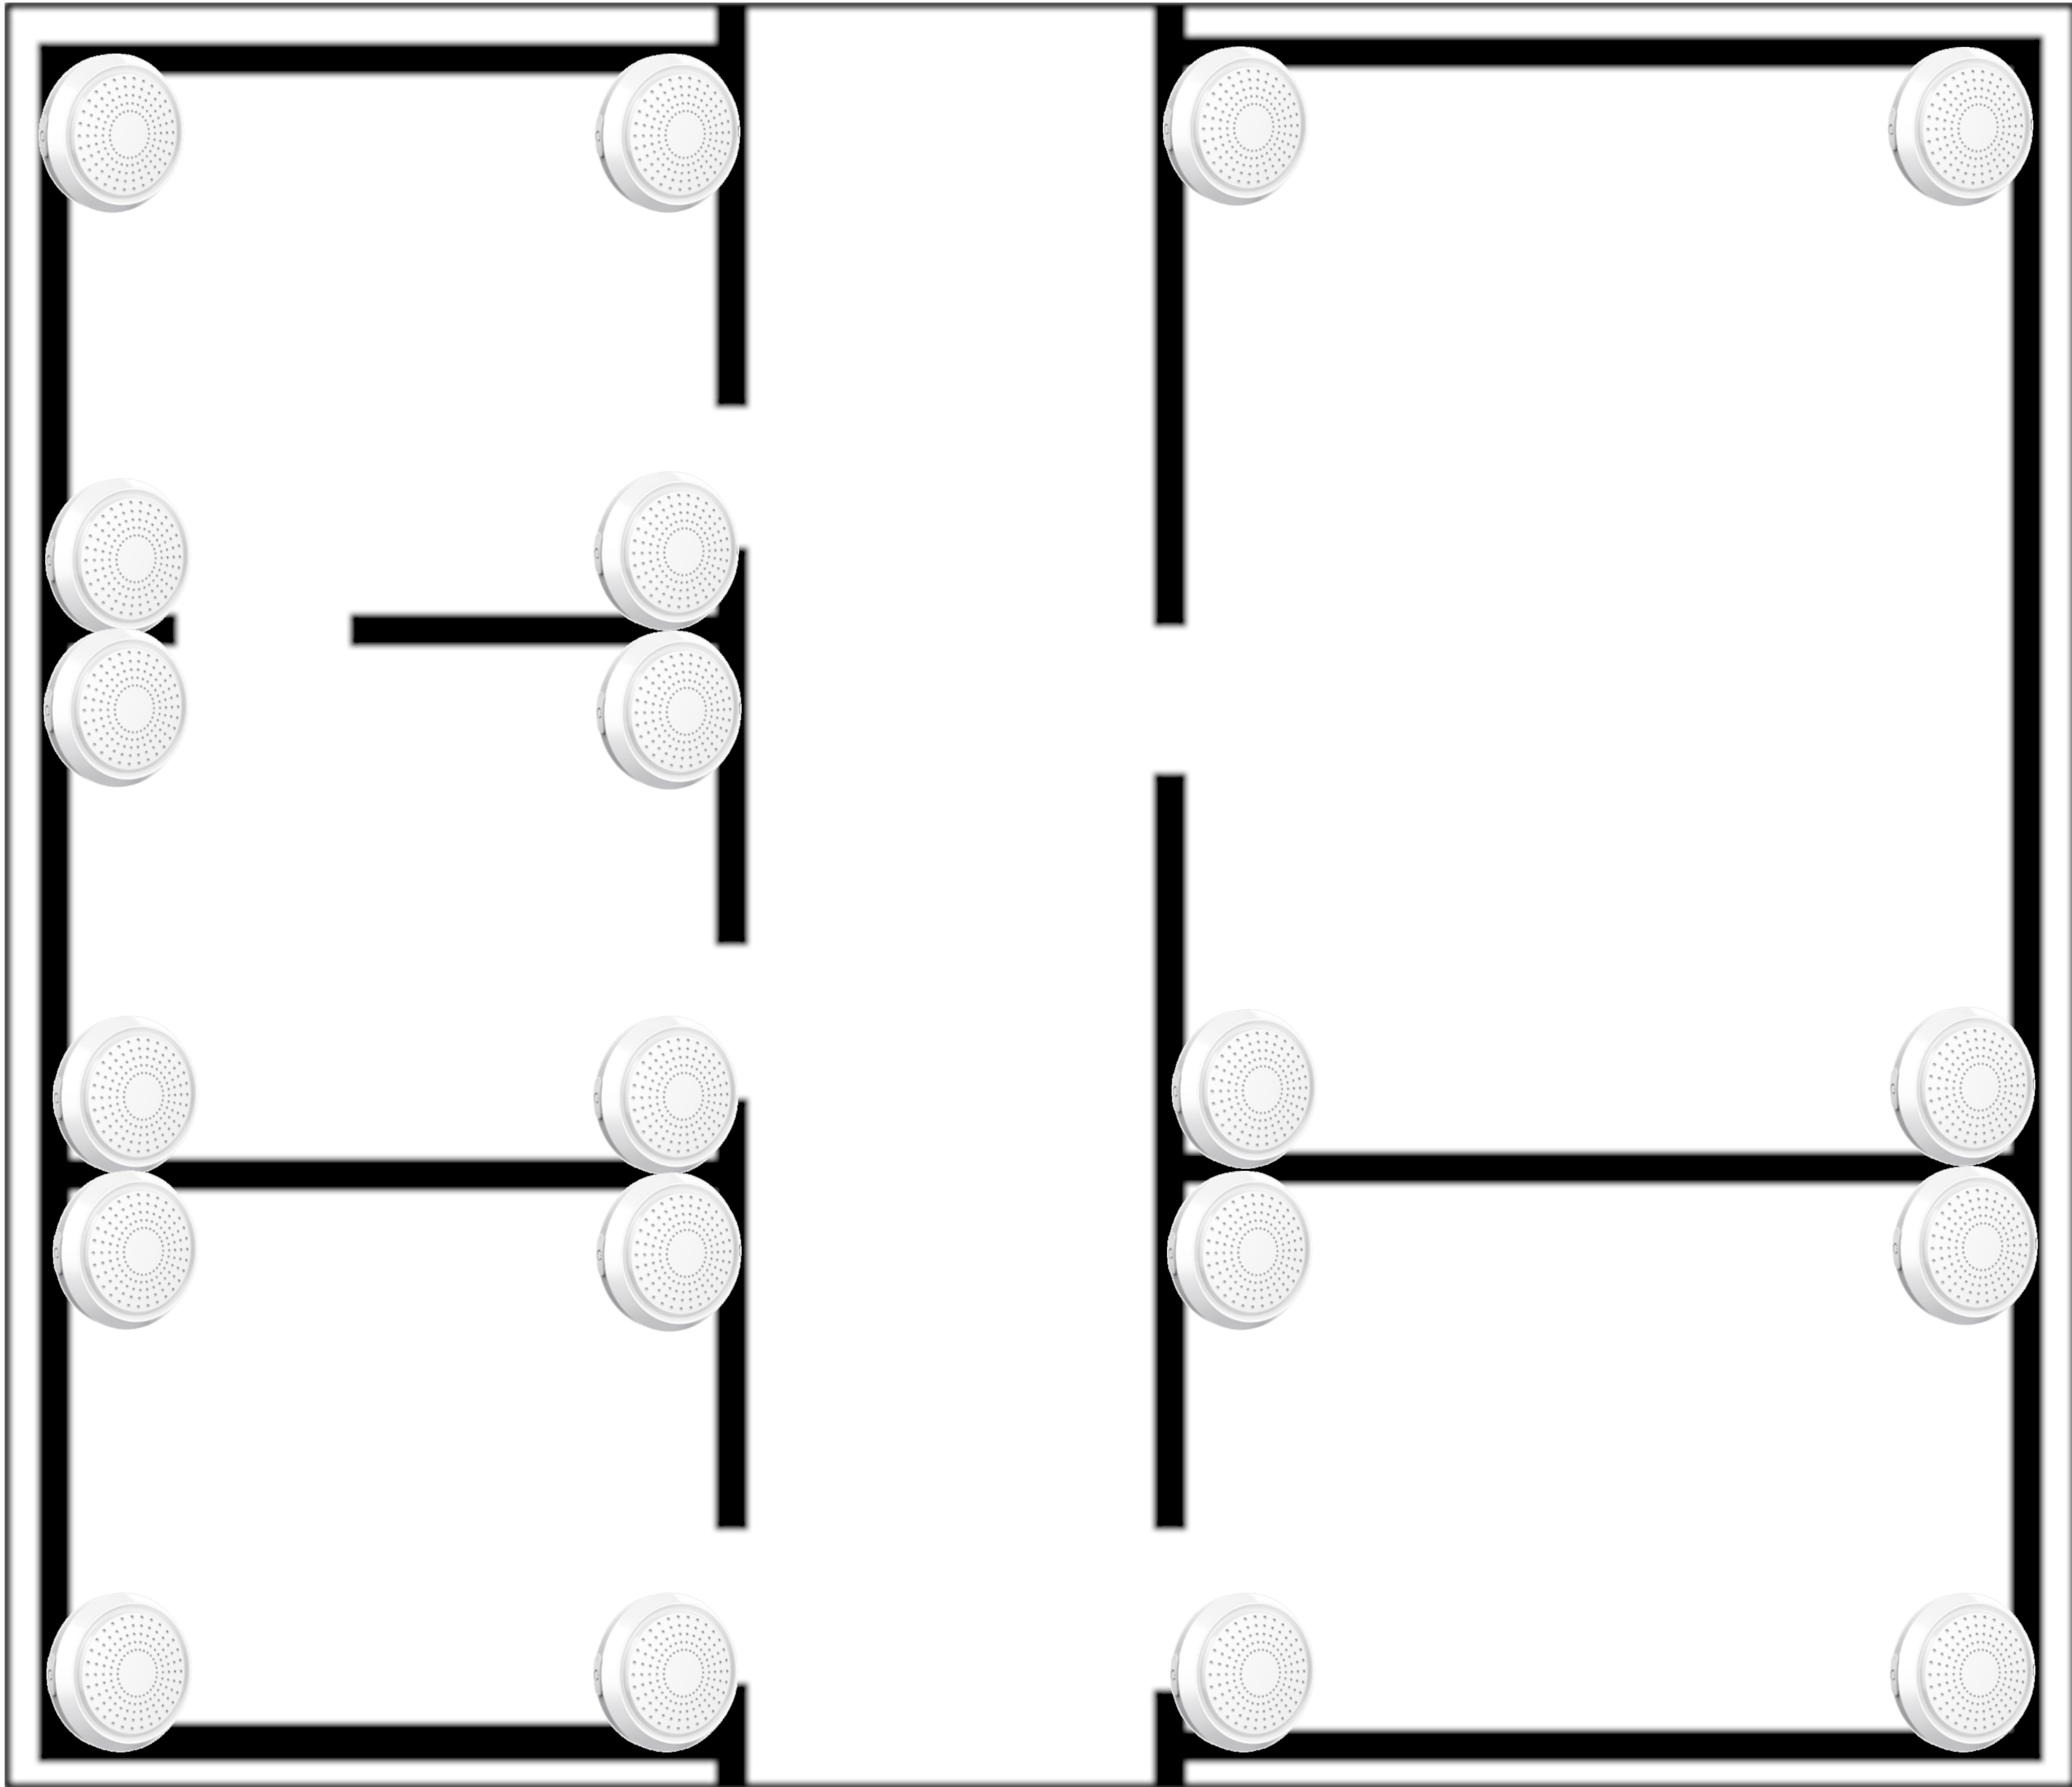
\includegraphics[width=\linewidth]{ble_dynamic_3}
	\captionof{figure}{Illustratie meerdere locatiebeacons per locatie}
	\label{fig:ops-ble-dynamic-3}
\end{minipage}

\subsubsection{Beacons in rasteropstelling}
\begin{minipage}{0.65\textwidth}
Dit is de dynamische tegenhanger van het 3e statische scenario, nl. een raster van locatiebeacons. In theorie kunnen hierbij de locaties van de assetbeacons bepaald worden door dubbele trilateratie, nl. de locatie van de mobiele gateway kan bepaald worden op 3 meetpunten a.d.h.v. de geweten locatie van de locatiebeacons, en uit deze 3 locaties kan dan nog eens via trilateratie de locatie van de assetbeacons worden bepaald. Het vermoeden bestaat echter dat dit onnauwkeurig kan zijn, verder wordt er ook verondersteld dat het asset niet beweegt tussen deze gebruikte meetpunten maar dit is bij uitbreiding voor elke dynamische opstelling zo. Deze opstelling staat geïllustreerd op figuur~\ref{fig:ops-ble-dynamic-4}.
\end{minipage}
\hfill
\begin{minipage}{0.30\textwidth}
	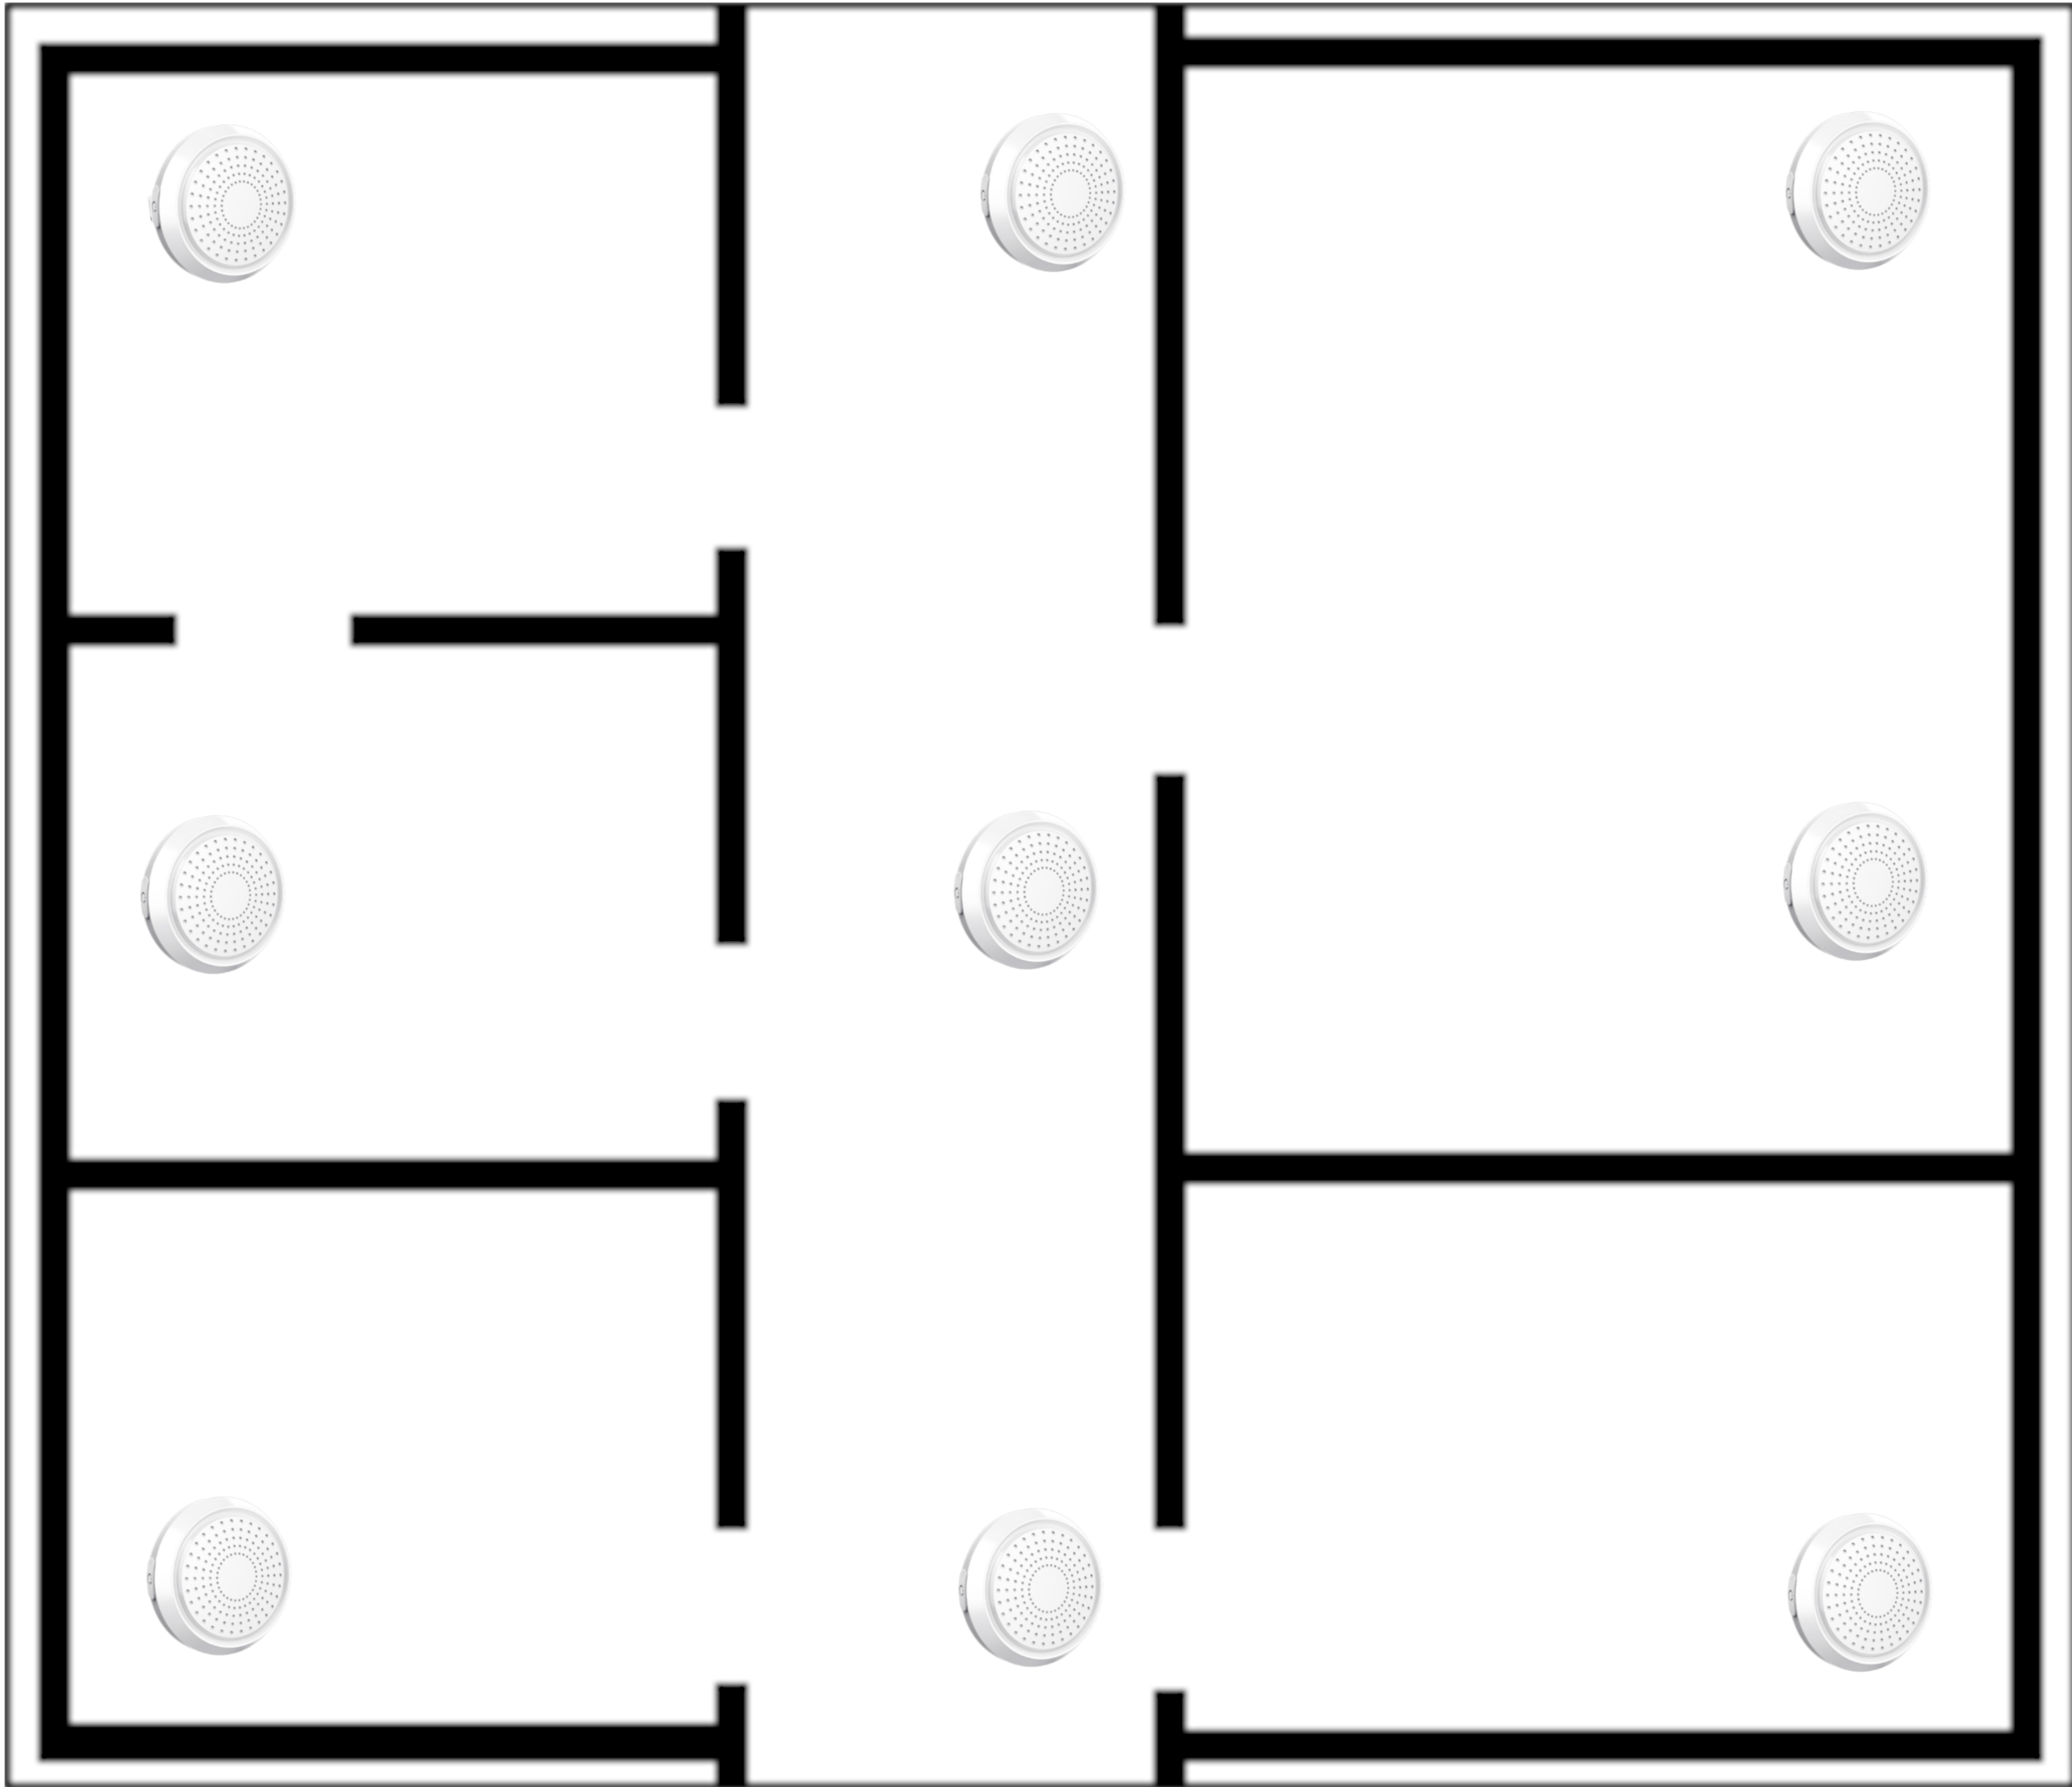
\includegraphics[width=\linewidth]{ble_dynamic_4}
	\captionof{figure}{Illustratie beacons in rasteropstelling}
	\label{fig:ops-ble-dynamic-4}
\end{minipage}

\subsubsection{Beacons op intervallen in de gang}
\begin{minipage}{0.65\textwidth}
Bij deze laatste opstelling worden er geen beacons in de locaties geplaatst, maar in de gang. Op deze manier worden de locaties en locatiebeacons 'ontkoppeld' en is er niet meer voor elke locatie een beacon nodig, wat kostendrukkend kan zijn. Deze locatiebeacons bevinden zich op constante intervallen van elkaar. In theorie weet de mobiele gateway hieraan waar hij zich bevind in de gang, als er geweten is op welke 'afstand' in de gang welke locatie zich bevind kan er bepaald worden welke assetbeacons zich op welke locatie bevinden. Deze opstelling staat geïllustreerd op figuur~\ref{fig:ops-ble-dynamic-5}.
\end{minipage}
\hfill
\begin{minipage}{0.30\textwidth}
	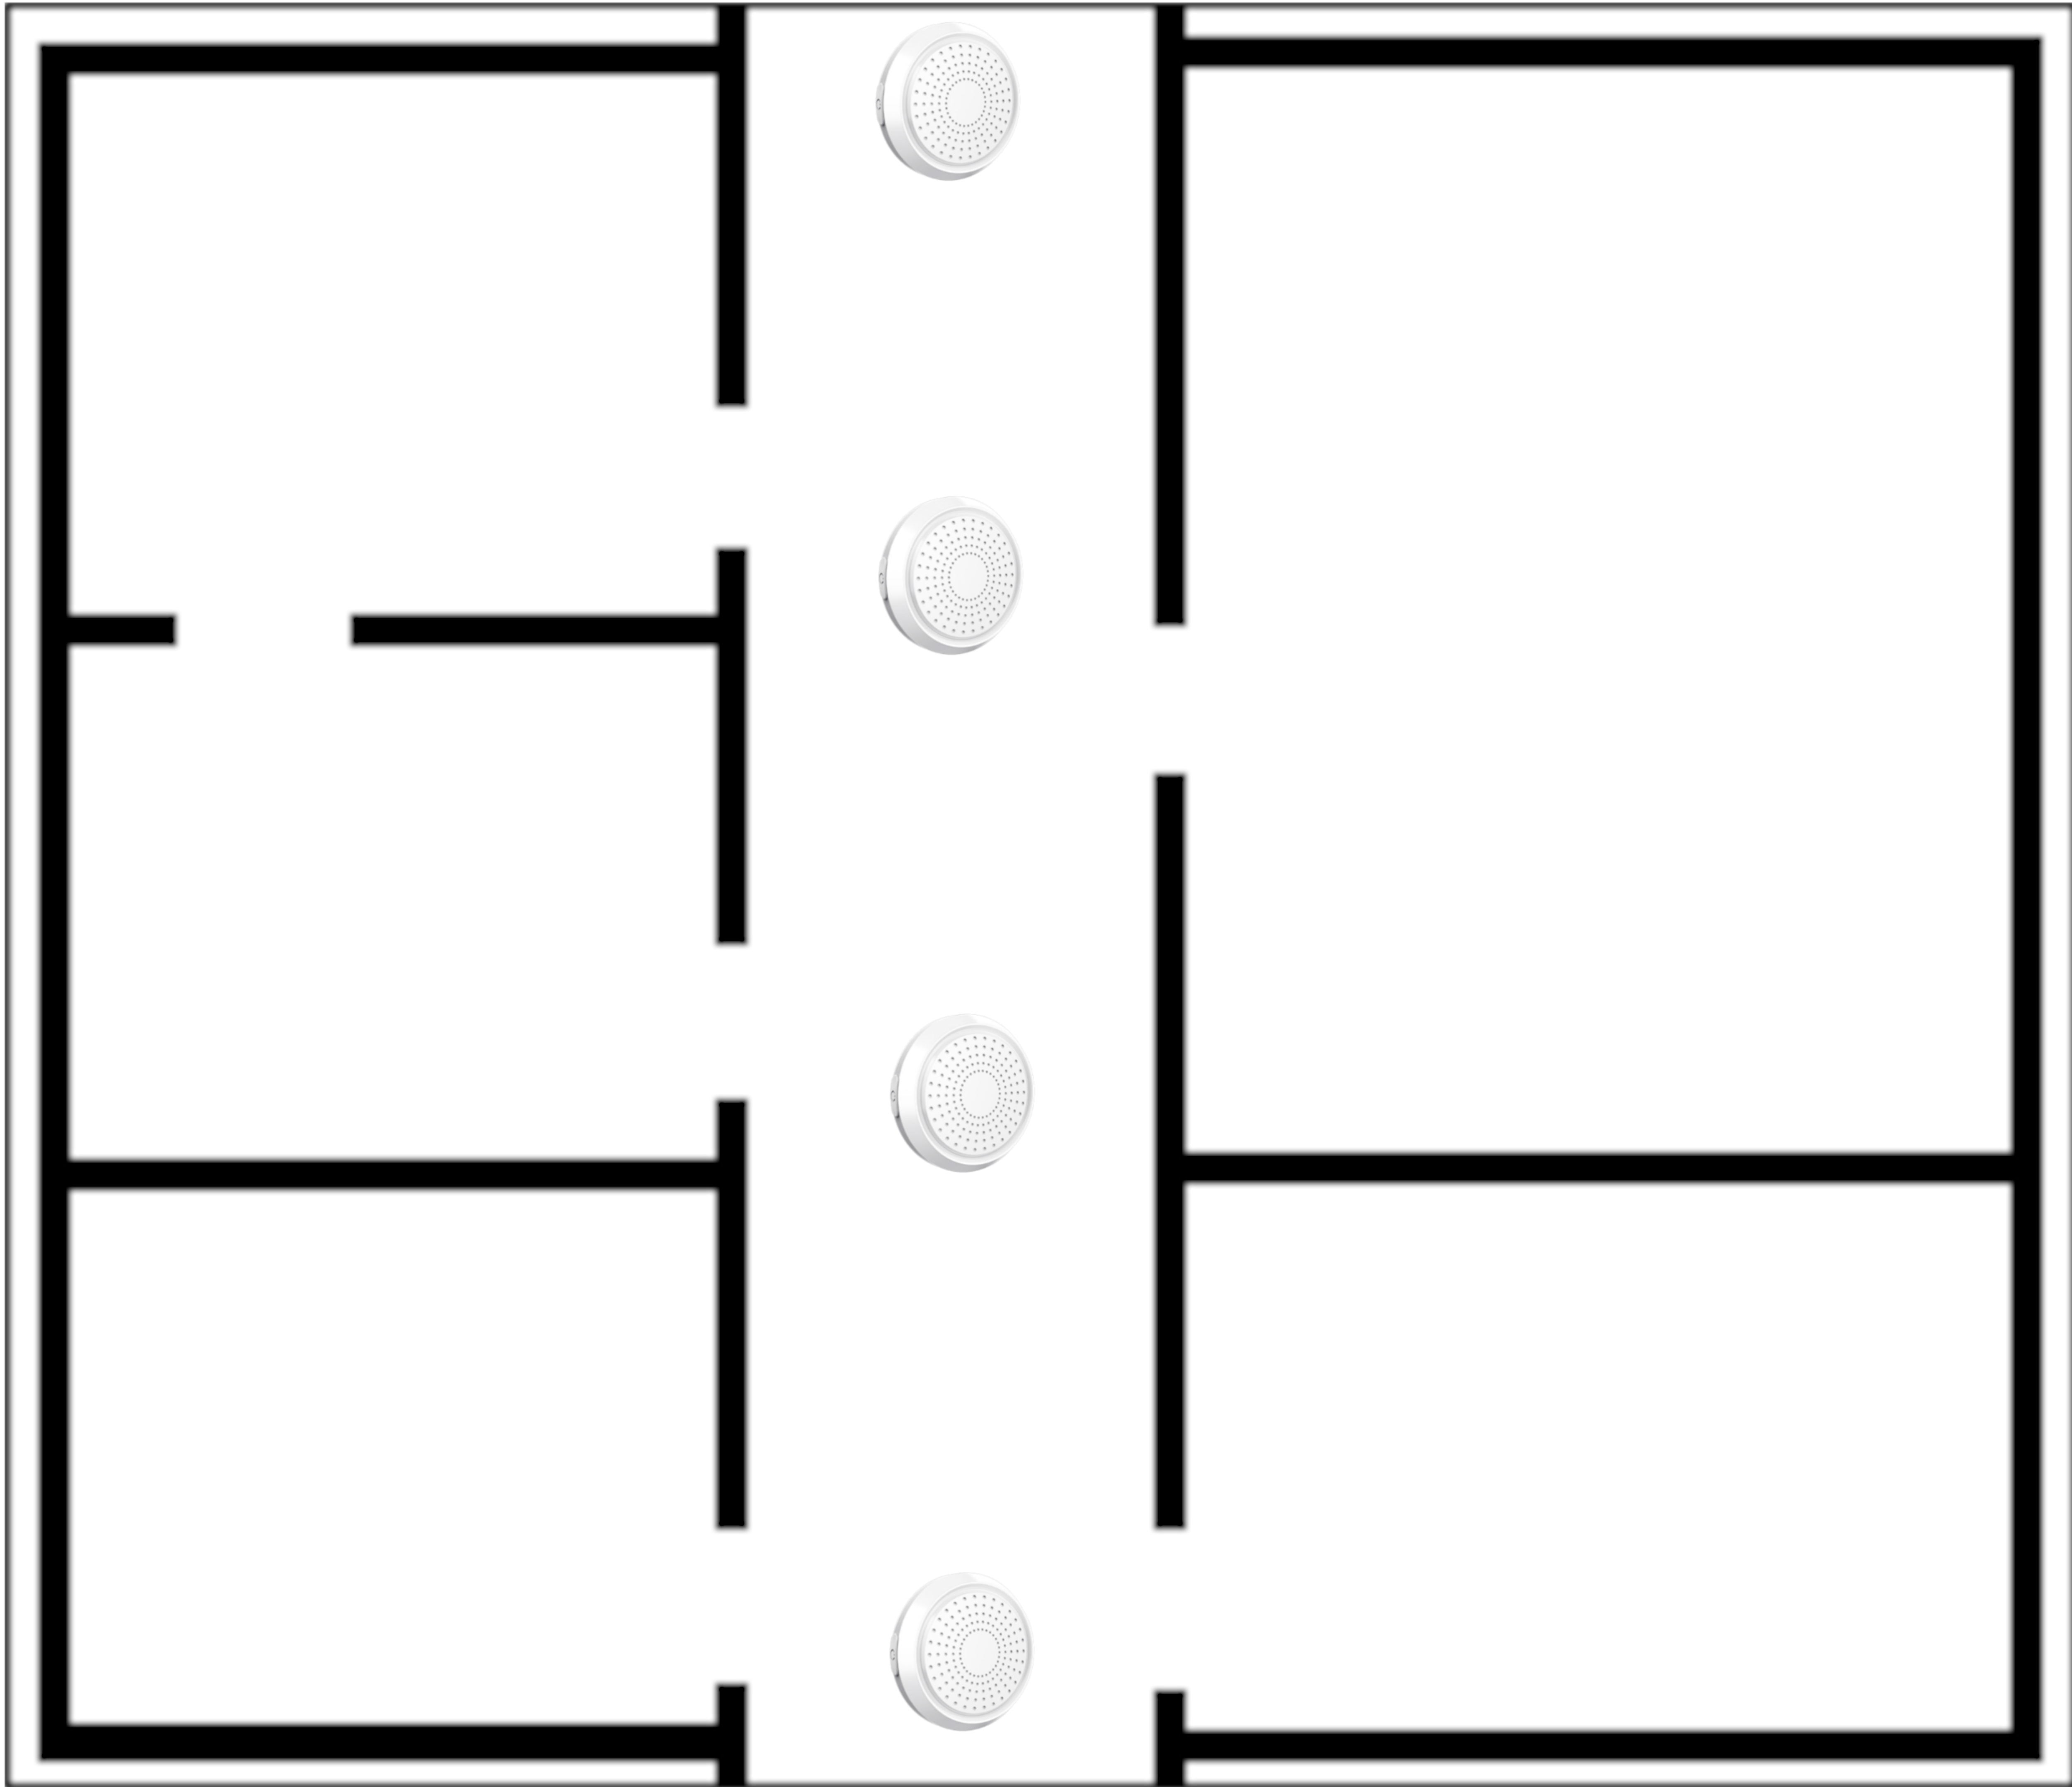
\includegraphics[width=\linewidth]{ble_dynamic_5}
	\captionof{figure}{Illustratie beacons op intervallen in de gang}
	\label{fig:ops-ble-dynamic-5}
\end{minipage}